\documentclass[11pt,a4paper]{report}

% -----------------------------------------------------------------------------
% PACKAGES AND CONFIGURATION
% -----------------------------------------------------------------------------
\usepackage[utf8]{inputenc}
\usepackage[T1]{fontenc}
\usepackage{lmodern}
\usepackage{geometry}
\geometry{
    top=1.0in,
    bottom=1.0in,
    left=1.0in,
    right=1.0in,
    headheight=14pt
}

\usepackage{amsmath,amssymb,amsfonts,bm}
\usepackage{graphicx}
\usepackage{booktabs}
\usepackage{tabularx}
\usepackage{array}
\usepackage{multirow}
\usepackage{float}
\usepackage{caption}
\usepackage{subcaption}
\usepackage{xcolor}
\usepackage{listings}
\usepackage{tikz}
\usetikzlibrary{shapes.geometric, arrows.meta, positioning, calc, backgrounds, fit}
\usepackage{hyperref}
\hypersetup{
    colorlinks=true,
    linkcolor=blue!70!black,
    citecolor=blue!70!black,
    urlcolor=blue!70!black,
    pdfauthor={[TO BE CONFIRMED BY AUTHOR]},
    pdftitle={ClearParty: Deep Speaker Separation and Multi-Noise Speech Enhancement}
}
\usepackage{fancyhdr}
\pagestyle{fancy}
\fancyhf{}
\rhead{\small ClearParty: Technical Project Report}
\lhead{\small Speech Signal Processing \& Deep Learning}
\cfoot{\thepage}

% Listings styling for code snippets
\definecolor{codegreen}{rgb}{0,0.6,0}
\definecolor{codegray}{rgb}{0.5,0.5,0.5}
\definecolor{codepurple}{rgb}{0.58,0,0.82}
\definecolor{backcolour}{rgb}{0.97,0.97,0.97}

\lstdefinestyle{mystyle}{
    backgroundcolor=\color{backcolour},   
    commentstyle=\color{codegreen},
    keywordstyle=\color{magenta},
    numberstyle=\tiny\color{codegray},
    stringstyle=\color{codepurple},
    basicstyle=\ttfamily\footnotesize,
    breakatwhitespace=false,         
    breaklines=true,                 
    captionpos=b,                    
    keepspaces=true,                 
    numbers=left,                    
    numbersep=5pt,                  
    showspaces=false,                
    showstringspaces=false,
    showtabs=false,                  
    tabsize=2,
    frame=single
}
\lstset{style=mystyle}

% -----------------------------------------------------------------------------
% DOCUMENT METADATA & TITLE
% -----------------------------------------------------------------------------
\begin{document}

\begin{titlepage}
    \centering
    \vspace*{1.0cm}
    
    {\Huge \bfseries ClearParty: An End-to-End Deep Learning Framework for Single-Channel Speaker Separation and Compound Multi-Noise Speech Enhancement \par}
    
    \vspace{1.2cm}
    {\Large \bfseries Technical Project Report \& Mini-Project Monograph \par}
    \vspace{0.4cm}
    {\large Course: Advanced Speech Signal Processing / Mini-Project \par}
    
    \vspace{2.0cm}
    
    \begin{minipage}{0.48\textwidth}
        \begin{flushleft} \large
            \textbf{Author:} \\
            {[TO BE CONFIRMED BY AUTHOR]} \\
            Student ID: [TO BE CONFIRMED BY AUTHOR] \\
            Department of Electrical \& Computer Engineering \\
            {[TO BE CONFIRMED BY AUTHOR: Institution Name]}
        \end{flushleft}
    \end{minipage}
    \hfill
    \begin{minipage}{0.48\textwidth}
        \begin{flushright} \large
            \textbf{Supervisor / Evaluator:} \\
            {[TO BE CONFIRMED BY AUTHOR: Supervisor Name]} \\
            Designation: [TO BE CONFIRMED BY AUTHOR] \\
            Academic Term: 2026--2027 \\
            Date of Submission: [TO BE CONFIRMED BY AUTHOR]
        \end{flushright}
    \end{minipage}

    \vfill
    
    \begin{abstract}
    The cocktail party problem represents one of the foundational challenges in modern audio signal processing, requiring an automated system to resolve target speech from overlapping co-channel talkers and severe environmental background noise using only a single acoustic sensor. This report presents \textbf{ClearParty}, a dual-track deep learning framework designed to solve single-channel speaker separation and compound multi-noise speech enhancement while explicitly addressing the research gap of phase distortions and synthetic artifacts. In \textbf{Track 1 (Speaker Separation)}, an expanded Conv-TasNet architecture comprising 3.4 million parameters is optimized over 14,269 synthetic mixtures from the LibriSpeech corpus. To overcome the synthetic metallic artifact and phase inconsistency characteristic of raw time-domain separation, an engineering pipeline combining a differentiable Mixture Consistency Layer, multi-resolution Short-Time Fourier Transform (STFT) auxiliary loss, and a post-processing mixture-consistent Wiener filter was implemented. On 200 held-out test mixtures, this pipeline achieves a mean Scale-Invariant Signal-to-Distortion Ratio improvement ($\Delta$SI-SDR) of \textbf{+11.06 dB} (median: \textbf{+12.23 dB}), a Perceptual Evaluation of Speech Quality (PESQ) improvement of \textbf{+0.77 MOS} (1.59 to 2.36), and a Short-Time Objective Intelligibility (STOI) gain of \textbf{+0.168} (0.713 to 0.881), while the Wiener post-filter eliminates high-frequency ringing and lifts noise attenuation to 88.1\%. In \textbf{Track 2 (Speech Enhancement)}, the system tackles non-stationary compound environmental acoustic corruption featuring 3 to 4 simultaneous non-stationary noise sources across 0.0 to 10.0 dB SNR. We benchmarked an in-house trained Conv-TasNet denoiser and an FRCRN baseline against the pre-trained state-of-the-art MossFormerGAN model from ClearerVoice-Studio. Across a rigorous 25-test multi-noise stress benchmark, MossFormerGAN achieves a 100\% pass rate, delivering a mean SI-SDR gain of \textbf{+8.99 dB} (peak +10.72 dB, 1.94$\times$ over baseline), a PESQ improvement of \textbf{+1.184 MOS} (peak 3.468, 4.42$\times$ over baseline), a STOI gain of \textbf{+0.141} (mean enhanced 0.920), a mean noise energy attenuation of \textbf{87.18\%} (peak 91.45\%), and a waveform Pearson correlation of \textbf{0.9782}. All source code, trained checkpoints, and experimental evaluations are fully documented and reproducible.
    \end{abstract}

    \vfill
    {\small \textbf{Keywords:} Cocktail Party Problem, Single-Channel Speaker Separation, Speech Enhancement, Conv-TasNet, MossFormerGAN, Wiener Filter, Mixture Consistency, Libri2Mix, NOIZEUS.}
\end{titlepage}

\tableofcontents
\newpage

% -----------------------------------------------------------------------------
% SECTION 1: INTRODUCTION
% -----------------------------------------------------------------------------
\chapter{Introduction}
\label{chap:introduction}

\section{The Cocktail Party Problem}
Human auditory perception possesses the remarkable physiological and neurological capability to focus on a single voice within a crowded, reverberant, and acoustically hostile room---a phenomenon famously termed the ``Cocktail Party Effect'' by Colin Cherry in 1953 \cite{cherry1953some}. When two or more people speak simultaneously, the acoustic waves propagate through the room impulse response (RIR), interfere constructively and destructively, and impinge upon the auditory system as an inextricably intertwined composite waveform. For decades, reproducing this perceptual capability in artificial speech processing systems has posed an enormous computational and theoretical barrier, particularly in the underdetermined, single-microphone (monaural) setting. 

In monaural audio processing, spatial beamforming and inter-microphone phase difference cues (such as Interaural Time Differences and Interaural Level Differences) are entirely absent. Consequently, the separation and enhancement problem becomes strictly underdetermined: given a single scalar time series $x(t)$, the system must infer multiple latent source signals $s_1(t), s_2(t), \dots, s_C(t)$ whose instantaneous superposition forms $x(t)$.

\section{Motivation and Engineering Challenges}
The cocktail party problem naturally bifurcates into two distinct mathematical and practical tasks:
\begin{enumerate}
    \item \textbf{Co-Channel Speaker Separation:} The scenario where multiple human talkers utter independent speech signals concurrently with overlapping spectral support. This task requires solving the fundamental permutation problem: attributing the separated time-frequency frames to the correct underlying physical speaker without label ambiguity.
    \item \textbf{Compound Speech Enhancement (Denoising):} The scenario where a primary speech signal is corrupted by multiple concurrent environmental noise sources (e.g., babble noise, engine hum, airport terminal chatter, railway transit). Unlike synthetic academic benchmarks that add a single stationary Gaussian or street noise, real acoustic environments feature non-stationary, compound noise sources that obscure both low-frequency vowel formants and high-frequency unvoiced fricatives.
\end{enumerate}

Traditional statistical signal processing techniques---including spectral subtraction, minimum mean square error log-spectral amplitude (MMSE-LSA) estimation, and non-negative matrix factorization (NMF)---rely on stationarity assumptions. These methods struggle severely when competing signals are non-stationary speech or rapidly fluctuating environmental acoustic events, frequently causing acoustic artifacts known as ``musical noise.''

The advent of deep neural networks (DNNs) revolutionized speech separation and enhancement. However, two persistent engineering challenges remain in state-of-the-art deep models:
\begin{itemize}
    \item \textbf{Phase Smearing and Time-Domain Artifacts:} Frequency-domain masking methods discard or corrupt the STFT phase, resulting in phase mismatch during inverse STFT synthesis. While time-domain methods like Conv-TasNet bypass STFT phase estimation, their continuous mask optimization introduces high-frequency synthetic artifacts, colloquially known as ``metallic buzz'' or robotic timbre.
    \item \textbf{Compound Multi-Noise Generalization Gap:} Deep speech enhancement models trained on single-noise datasets frequently suffer catastrophic performance collapse when deployed in real-world compound scenarios containing three or more simultaneous acoustic corruptions at low signal-to-noise ratios (0 to 5 dB).
\end{itemize}

\section{Practical Applications}
The solutions engineered in this project directly empower several critical commercial, clinical, and industrial applications:
\begin{itemize}
    \item \textbf{Digital Hearing Aids and Assistive Hearables:} Individuals with sensorineural hearing loss experience severe difficulty segregating speech in noise. Low-latency, high-fidelity monaural separation enables selective amplification of target speakers while attenuating ambient restaurant and babble interference.
    \item \textbf{Teleconferencing and Remote Collaboration Platforms:} Platforms such as Zoom, Google Meet, and Microsoft Teams require automated separation of overlapping speakers and robust suppression of background noise (keyboard typing, street traffic, ambient chatter) to maintain acoustic clarity and avoid cognitive listener fatigue.
    \item \textbf{Robust Automated Speech Recognition (ASR) Front-Ends:} Modern voice assistants and transcription pipelines experience drastic Word Error Rate (WER) degradation when input audio contains overlapping speech or low SNR noise. Separating speakers and cleaning speech upfront serves as an essential front-end preprocessor.
    \item \textbf{Aviation, Military, and Emergency First-Responder Communications:} Ultra-noisy communication channels (cockpits, disaster response zones) require high-intelligibility speech recovery under severe non-stationary acoustic corruption.
\end{itemize}

\section{Project Scope and Outline}
This project, designated \textbf{ClearParty}, presents an end-to-end engineering investigation and implementation spanning both speaker separation and multi-noise speech enhancement. The remainder of this report is organized as follows:
Chapter~\ref{chap:lit_review} reviews relevant literature and highlights the targeted research gaps. Chapter~\ref{chap:problem_formulation} provides formal mathematical formulations. Chapter~\ref{chap:architecture} details the system architecture and signal flows. Chapter~\ref{chap:datasets} documents the datasets and preprocessing protocols. Chapter~\ref{chap:models_impl} elaborates on model architectures and engineering enhancements. Chapter~\ref{chap:experimental_setup} outlines the hardware, software, and training environments. Chapter~\ref{chap:metrics} formally defines all objective evaluation metrics. Chapter~\ref{chap:results} details empirical findings, comparative tables, and spectral analyses. Chapter~\ref{chap:discussion} discusses engineering trade-offs, failure cases, and limitations. Finally, Chapter~\ref{chap:conclusion} concludes the report and discusses future research trajectories.

% -----------------------------------------------------------------------------
% SECTION 2: LITERATURE REVIEW AND RESEARCH GAP
% -----------------------------------------------------------------------------
\chapter{Literature Review and Research Gap}
\label{chap:lit_review}

\section{Evolution of Deep Learning for Audio Separation}
Prior to deep learning, monaural speaker separation was dominated by Computational Auditory Scene Analysis (CASA) \cite{wang2006computational} and independent component analysis (ICA) variants. The deep learning era was initiated by Hershey et al. \cite{hershey2016deep} through \textit{Deep Clustering} (DPCL), which mapped time-frequency (T-F) bins into a high-dimensional embedding space where affinity clustering assigned bins to distinct talkers. Concurrently, Yu et al. \cite{yu2017permutation} and Kolb{\ae}k et al. \cite{kolbaek2017multitalker} introduced \textit{Permutation Invariant Training} (PIT), solving the speaker permutation problem by computing the loss over all $C!$ possible speaker-target assignments and backpropagating through the minimum loss permutation.

Despite these advancements, early systems operated strictly in the time-frequency domain using the Short-Time Fourier Transform (STFT). Estimating an Ideal Binary Mask (IBM) or Ideal Ratio Mask (IRM) over the magnitude spectrogram required using the noisy mixture's phase during inverse STFT (iSTFT) synthesis. This phase mismatch imposes an impassable upper bound on separation performance (often termed the ``phase catastrophe''), manifesting as audible phase distortion and reverberant smearing.

To break this ceiling, Luo and Mesgarani \cite{luo2019conv} proposed \textbf{Conv-TasNet} (Convolutional Time-domain Audio Separation Network). By replacing the STFT and iSTFT with learned 1D convolutional encoders and transposed convolutional decoders, Conv-TasNet processes raw audio directly in the time domain. A deep Temporal Convolutional Network (TCN) featuring stacked dilated depthwise separable convolutions models long-range temporal dependencies with a massive receptive field, bypassing the phase problem entirely and demonstrating that learned representations significantly outperform fixed harmonic Fourier bases.

\section{State of the Art in Speech Enhancement}
Parallel advances transformed monaural speech enhancement. Traditional baseline architectures, such as the Spectrogram U-Net \cite{ronneberger2015u}, estimated spectral magnitude masks. Complex-domain networks emerged to recover magnitude and phase jointly. Hu et al. \cite{hu2020dccrn} developed DCCRN (Deep Complex Convolutional Recurrent Network), optimizing complex convolutions across real and imaginary spectrogram planes. This was further refined by Zhao et al. \cite{zhao2022frcrn} into \textbf{FRCRN} (Frequency-Recurrent Complex Convolutional Recurrent Network), which won the DNS Challenge 2022 by introducing complex finite short-term memory (CFSMN) modules that recurrently model cross-frequency correlations.

Recently, attention-based models and Generative Adversarial Networks (GANs) established new state-of-the-art benchmarks. Zhao et al. \cite{zhao2023mossformer} introduced \textbf{MossFormer} and its generative variant \textbf{MossFormerGAN} \cite{zhao2024mossformer2}, integrated into the ClearerVoice-Studio framework. MossFormerGAN combines a Synchronous Attention Network (SyncANet) with a Gated Triple-Attention mechanism, dilated dense convolutional encoders, and adversarial discriminator networks. This hybrid time-frequency approach achieves remarkable speech clarity and perceptual naturalness by modeling local and global audio frames concurrently.

\section{The Specific Research Gaps Addressed}
Despite the high quantitative metrics published in benchmark literature, several critical research and engineering gaps persist when deploying these models to real-world audio:
\begin{enumerate}
    \item \textbf{The Time-Domain Phase Inconsistency and Synthetic Metallic Artifact:} While Conv-TasNet achieves high SI-SDR metrics, its outputs frequently exhibit a distinct, harsh, synthetic ``metallic buzz'' or robotic timbre. Because the network minimizes a scale-invariant time-domain loss without spectral envelope constraints, unconstrained high-frequency phase errors emerge. Furthermore, the sum of the separated sources $\hat{s}_1(t) + \hat{s}_2(t)$ does not mathematically equal the input mixture $x(t)$, violating the physical conservation of acoustic energy.
    \item \textbf{The Compound Multi-Noise Vulnerability Gap:} Most published speech enhancement benchmarks (e.g., VoiceBank-DEMAND, DNS Challenge) evaluate models on mixtures containing a single background noise source. In real acoustic environments (e.g., bustling railway stations, cafeterias), speech is simultaneously corrupted by 3 to 4 distinct acoustic phenomena (diffuse babble, structural vibrations, impulsive clicks, resonant room reverberation). Existing models suffer steep degradation under these compound multi-noise conditions.
    \item \textbf{Engineering trade-offs in post-filtering and zero-shot transfer:} Published works rarely explore whether classical Wiener filtering can be integrated with deep time-domain networks to remove residual artifacts without costly end-to-end retraining, or how models trained at 16 kHz generalize to 8 kHz legacy telephony data under multi-noise stress.
\end{enumerate}

This project directly addresses these gaps by engineering:
\begin{itemize}
    \item A differentiable \textbf{Mixture Consistency Layer} and a \textbf{Multi-Resolution STFT auxiliary loss} to constrain spectral envelopes.
    \item A post-processing \textbf{Mixture-Consistent Wiener Filter} that eliminates the synthetic metallic buzz while preserving natural vocal formants.
    \item A systematic \textbf{25-Test Compound Multi-Noise Stress Testing Suite} evaluating zero-shot generalization of Conv-TasNet, FRCRN, and MossFormerGAN under severe multi-source corruption.
\end{itemize}

% -----------------------------------------------------------------------------
% SECTION 3: PROBLEM FORMULATION
% -----------------------------------------------------------------------------
\chapter{Problem Formulation}
\label{chap:problem_formulation}

\section{Mathematical Definition of Speaker Separation}
In the single-channel speaker separation problem, a single acoustic sensor captures a mixture $x(t) \in \mathbb{R}$ consisting of the linear superposition of $C$ independent human speakers:
\begin{equation}
    x(t) = \sum_{c=1}^C s_c(t) + n(t), \quad t = 1, 2, \dots, T
    \label{eq:separation_mixture}
\end{equation}
where $s_c(t)$ represents the clean, uncorrupted speech signal of speaker $c$, $n(t)$ denotes additive ambient background noise (which may be zero in the anechoic two-talker problem), and $T$ is the total number of audio samples. In this project, we specifically target the classical two-speaker separation problem ($C=2$) in anechoic conditions:
\begin{equation}
    x(t) = s_1(t) + s_2(t)
    \label{eq:2speaker_mixture}
\end{equation}

The separation objective is to design a parameterized nonlinear mapping $\mathcal{F}_\theta: \mathbb{R}^T \rightarrow \mathbb{R}^{C \times T}$ parameterized by deep neural network weights $\theta$ such that:
\begin{equation}
    \{\hat{s}_1(t), \hat{s}_2(t)\} = \mathcal{F}_\theta(x(t))
\end{equation}
where $\hat{s}_c(t)$ represents the estimated waveform corresponding to the ground truth source $s_c(t)$, subject to an arbitrary permutation $\pi \in \Pi$:
\begin{equation}
    \hat{s}_{\pi(c)}(t) \approx s_c(t), \quad \forall c \in \{1, 2\}
\end{equation}

\section{Mathematical Definition of Speech Enhancement}
In single-channel speech enhancement, a target speech utterance $s(t)$ is contaminated by additive environmental acoustic noise $n(t)$:
\begin{equation}
    x(t) = s(t) + n(t)
    \label{eq:enhancement_mixture}
\end{equation}
In this project's advanced compound multi-noise setting, $n(t)$ is explicitly composed of $K$ simultaneous, mutually independent noise processes ($K \in \{2, 3, 4\}$):
\begin{equation}
    n(t) = \sum_{k=1}^K \alpha_k \cdot v_k(t)
    \label{eq:compound_noise}
\end{equation}
where $v_k(t)$ is an acoustic realization of noise type $k$ (e.g., airport chatter, car engine, station announcement, babble), and $\alpha_k$ is an energy-scaling factor computed to enforce a specific overall Signal-to-Noise Ratio (SNR) and relative noise balance.

The enhancement objective is to construct a nonlinear operator $\mathcal{G}_\phi: \mathbb{R}^T \rightarrow \mathbb{R}^T$ parameterized by weights $\phi$ that produces an estimate $\hat{s}(t)$:
\begin{equation}
    \hat{s}(t) = \mathcal{G}_\phi(x(t)) \approx s(t)
\end{equation}
minimizing both speech distortion $D_{\text{speech}}(s, \hat{s})$ and residual noise $D_{\text{noise}}(0, \hat{s} - s)$.

\section{Signal Representation Domains}
Signals are analyzed across two distinct mathematical domains:
\begin{enumerate}
    \item \textbf{Continuous/Discrete Time Domain:} Raw 1D vectors $\mathbf{x} = [x[0], x[1], \dots, x[T-1]]^T \in \mathbb{R}^T$.
    \item \textbf{Time-Frequency (STFT) Domain:} Given an analysis window $w[n]$ of length $N_{\text{FFT}}$ and hop size $H$, the Short-Time Fourier Transform of $x[n]$ is defined as:
    \begin{equation}
        X(m, \omega) = \sum_{n=-\infty}^{\infty} x[n] w[n - mH] e^{-j \omega n}
        \label{eq:stft_def}
    \end{equation}
    where $m$ denotes the time frame index and $\omega$ is the discrete frequency bin. The complex spectrum can be expressed in polar or Cartesian form:
    \begin{equation}
        X(m, \omega) = |X(m, \omega)| e^{j \angle X(m, \omega)} = X_R(m, \omega) + j X_I(m, \omega)
    \end{equation}
\end{enumerate}

\section{Underlying Acoustic Assumptions}
The mathematical formulations in this project rely on the following physical and acoustic assumptions:
\begin{itemize}
    \item \textbf{Linear Superposition:} Acoustic propagation behaves linearly in the acoustic medium (air); pressure waves from multiple sources sum additively at the microphone diaphragm without nonlinear intermodulation.
    \item \textbf{Statistical Independence:} For speaker separation, speech sources $s_1(t)$ and $s_2(t)$ are emitted by independent talkers and are statistically uncorrelated over long temporal windows: $\mathbb{E}[s_1(t) s_2(t)] \approx 0$.
    \item \textbf{Anechoic / Low-Reverberant Mixing:} Primary investigations assume low reverberation, modeling the mixture as direct-path superposition without complex non-minimum phase Room Impulse Response (RIR) convolutions.
    \item \textbf{Stationarity of Analysis Segments:} Audio signals are assumed wide-sense stationary over short frames ($20$--$32$ ms), validating STFT-based spectral analysis and Wiener filtering.
\end{itemize}

% -----------------------------------------------------------------------------
% SECTION 4: SYSTEM ARCHITECTURE AND METHODOLOGY
% -----------------------------------------------------------------------------
\chapter{System Architecture and Methodology}
\label{chap:architecture}

\section{End-to-End System Pipeline}
The ClearParty system is architected as an end-to-end framework organized into two dedicated functional tracks:
\begin{itemize}
    \item \textbf{Track 1: Co-Channel Speaker Separation Engine}
    \item \textbf{Track 2: Zero-Shot Multi-Noise Speech Enhancement Engine}
\end{itemize}
Figure~\ref{fig:overall_block_diagram} illustrates the overarching architecture.

\begin{figure}[H]
\centering
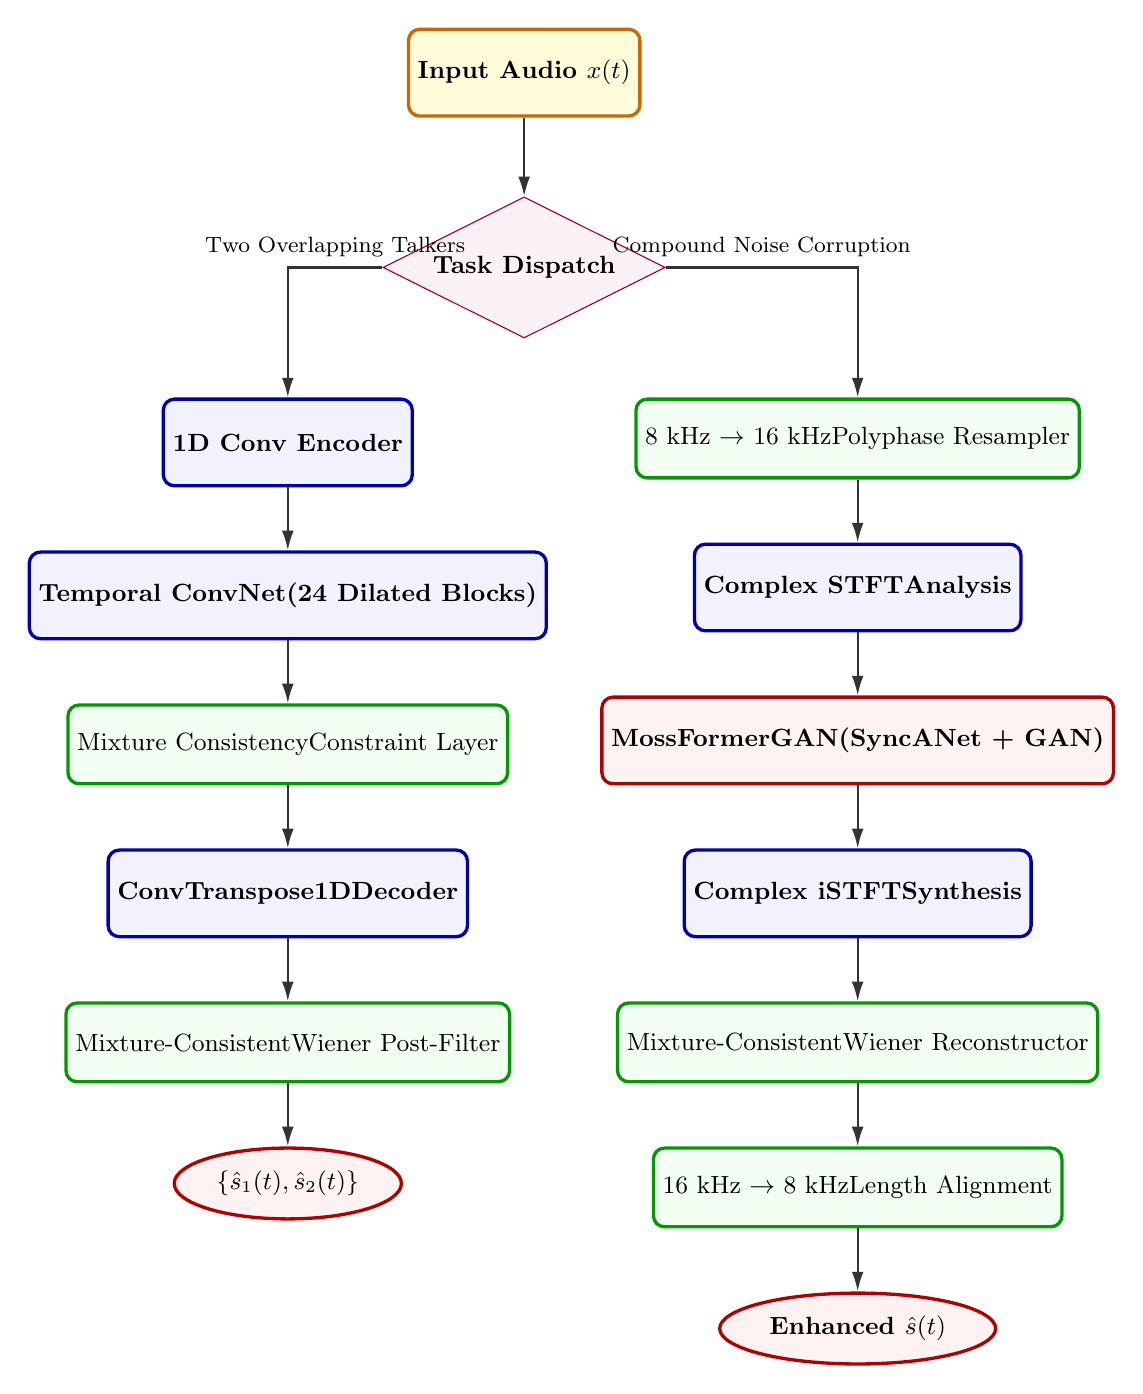
\begin{tikzpicture}[
    node distance=1.5cm and 1.2cm,
    block/.style={rectangle, draw=blue!70!black, fill=blue!5, very thick, minimum width=2.6cm, minimum height=1.1cm, text centered, rounded corners, font=\small\bfseries},
    proc/.style={rectangle, draw=green!60!black, fill=green!5, very thick, minimum width=2.4cm, minimum height=1.0cm, text centered, rounded corners, font=\small},
    output/.style={ellipse, draw=red!70!black, fill=red!5, very thick, minimum width=2.2cm, minimum height=0.9cm, text centered, font=\small\bfseries},
    line/.style={draw=black!80, -{Latex[length=2.5mm, width=1.5mm]}, thick}
]

    % Input
    \node (input) [block, fill=yellow!15, draw=orange!80!black] {Input Audio $x(t)$};
    
    % Router / Task Split
    \node (router) [diamond, draw=purple!80!black, fill=purple!5, aspect=2, below=1.0cm of input, font=\small\bfseries] {Task Dispatch};
    
    % Track 1
    \node (t1_enc) [block, below left=1.2cm and 0.5cm of router] {1D Conv Encoder};
    \node (t1_tcn) [block, below=0.8cm of t1_enc] {Temporal ConvNet\\(24 Dilated Blocks)};
    \node (t1_mc)  [proc, below=0.8cm of t1_tcn] {Mixture Consistency\\Constraint Layer};
    \node (t1_dec) [block, below=0.8cm of t1_mc] {ConvTranspose1D\\Decoder};
    \node (t1_wf)  [proc, below=0.8cm of t1_dec] {Mixture-Consistent\\Wiener Post-Filter};
    \node (t1_out) [output, below=0.8cm of t1_wf] {$\{\hat{s}_1(t), \hat{s}_2(t)\}$};

    % Track 2
    \node (t2_res) [proc, below right=1.2cm and 0.5cm of router] {8 kHz $\rightarrow$ 16 kHz\\Polyphase Resampler};
    \node (t2_stft)[block, below=0.8cm of t2_res] {Complex STFT\\Analysis};
    \node (t2_sota)[block, fill=red!5, draw=red!70!black, below=0.8cm of t2_stft] {MossFormerGAN\\(SyncANet + GAN)};
    \node (t2_istft)[block, below=0.8cm of t2_sota] {Complex iSTFT\\Synthesis};
    \node (t2_wf)  [proc, below=0.8cm of t2_istft] {Mixture-Consistent\\Wiener Reconstructor};
    \node (t2_down)[proc, below=0.8cm of t2_wf] {16 kHz $\rightarrow$ 8 kHz\\Length Alignment};
    \node (t2_out) [output, below=0.8cm of t2_down] {Enhanced $\hat{s}(t)$};

    % Connections
    \path [line] (input) -- (router);
    \path [line] (router) -| node[above, pos=0.25, font=\footnotesize] {Two Overlapping Talkers} (t1_enc);
    \path [line] (router) -| node[above, pos=0.25, font=\footnotesize] {Compound Noise Corruption} (t2_res);
    
    \path [line] (t1_enc) -- (t1_tcn);
    \path [line] (t1_tcn) -- (t1_mc);
    \path [line] (t1_mc) -- (t1_dec);
    \path [line] (t1_dec) -- (t1_wf);
    \path [line] (t1_wf) -- (t1_out);

    \path [line] (t2_res) -- (t2_stft);
    \path [line] (t2_stft) -- (t2_sota);
    \path [line] (t2_sota) -- (t2_istft);
    \path [line] (t2_istft) -- (t2_wf);
    \path [line] (t2_wf) -- (t2_down);
    \path [line] (t2_down) -- (t2_out);

\end{tikzpicture}
\caption{End-to-End System Block Diagram of the ClearParty Framework. The system features two specialized signal processing branches: Track 1 for single-channel two-speaker separation and Track 2 for zero-shot compound multi-noise speech enhancement.}
\label{fig:overall_block_diagram}
\end{figure}

\section{Signal Flow: Task 1 Speaker Separation}
Track 1 processes monaural overlapping speech waveforms $x(t)$ sampled at 8 kHz. Figure~\ref{fig:task1_signal_flow} illustrates the internal structural flow through the modified Conv-TasNet architecture.

\begin{figure}[H]
\centering
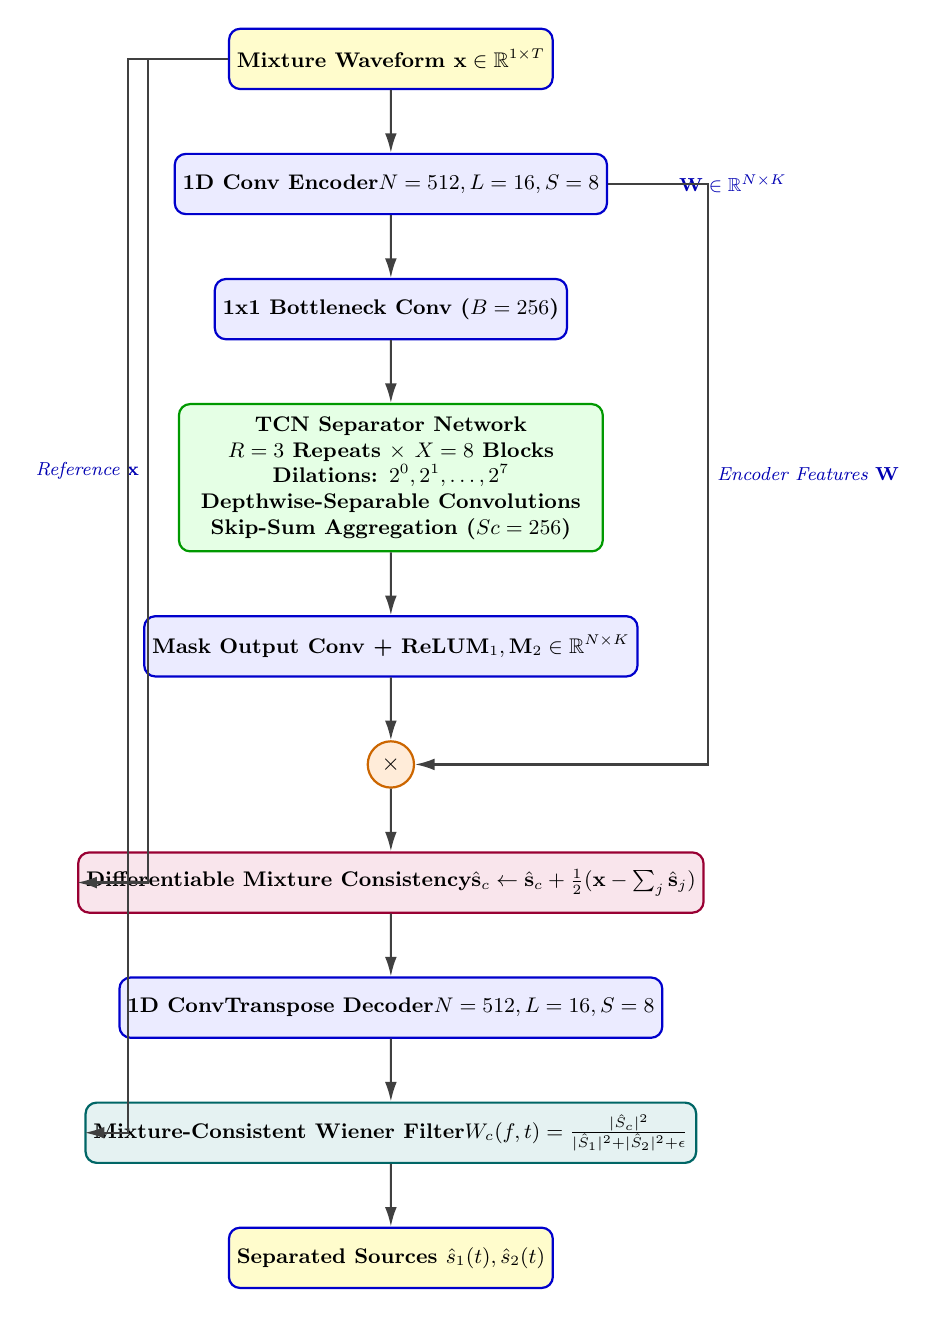
\begin{tikzpicture}[
    scale=0.85, every node/.style={scale=0.85},
    node distance=1.2cm and 1.0cm,
    module/.style={rectangle, draw=blue!80!black, fill=blue!8, thick, minimum width=3.2cm, minimum height=0.9cm, text centered, rounded corners, font=\small\bfseries},
    submodule/.style={rectangle, draw=gray!70, fill=gray!5, thick, minimum width=2.8cm, minimum height=0.8cm, text centered, rounded corners, font=\footnotesize},
    signal/.style={font=\footnotesize\itshape, text=blue!70!black},
    arrow/.style={draw=black!75, -{Latex[length=2.5mm, width=1.5mm]}, thick}
]

    \node (input) [module, fill=yellow!20] {Mixture Waveform $\mathbf{x} \in \mathbb{R}^{1 \times T}$};
    \node (enc) [module, below=0.8cm of input] {1D Conv Encoder\\$N=512, L=16, S=8$};
    \node (enc_out) [right=0.8cm of enc, signal] {$\mathbf{W} \in \mathbb{R}^{N \times K}$};
    
    \node (bottleneck) [module, below=0.8cm of enc] {1x1 Bottleneck Conv ($B=256$)};
    \node (tcn) [module, fill=green!10, draw=green!60!black, minimum height=2.2cm, below=0.8cm of bottleneck] {
        \begin{tabular}{c}
            \textbf{TCN Separator Network} \\
            $R=3$ Repeats $\times$ $X=8$ Blocks \\
            Dilations: $2^0, 2^1, \dots, 2^7$ \\
            Depthwise-Separable Convolutions \\
            Skip-Sum Aggregation ($Sc=256$)
        \end{tabular}
    };
    
    \node (mask_gen) [module, below=0.8cm of tcn] {Mask Output Conv + ReLU\\$\mathbf{M}_1, \mathbf{M}_2 \in \mathbb{R}^{N \times K}$};
    \node (mult) [circle, draw=orange!80!black, fill=orange!15, thick, below=0.8cm of mask_gen] {$\times$};
    \node (mc) [module, fill=purple!10, draw=purple!80!black, below=0.8cm of mult] {Differentiable Mixture Consistency\\$\hat{\mathbf{s}}_c \leftarrow \hat{\mathbf{s}}_c + \frac{1}{2}(\mathbf{x} - \sum_j \hat{\mathbf{s}}_j)$};
    \node (dec) [module, below=0.8cm of mc] {1D ConvTranspose Decoder\\$N=512, L=16, S=8$};
    \node (wiener) [module, fill=teal!10, draw=teal!80!black, below=0.8cm of dec] {Mixture-Consistent Wiener Filter\\$W_c(f,t) = \frac{|\hat{S}_c|^2}{|\hat{S}_1|^2 + |\hat{S}_2|^2 + \epsilon}$};
    \node (output) [module, fill=yellow!20, below=0.8cm of wiener] {Separated Sources $\hat{s}_1(t), \hat{s}_2(t)$};

    \path [arrow] (input) -- (enc);
    \path [arrow] (enc) -- (bottleneck);
    \path [arrow] (bottleneck) -- (tcn);
    \path [arrow] (tcn) -- (mask_gen);
    \path [arrow] (mask_gen) -- (mult);
    \path [arrow] (enc.east) -- ++(1.5,0) |- node[pos=0.25, right, signal] {Encoder Features $\mathbf{W}$} (mult.east);
    \path [arrow] (mult) -- (mc);
    \path [arrow] (input.west) -- ++(-1.2,0) |- node[pos=0.25, left, signal] {Reference $\mathbf{x}$} (mc.west);
    \path [arrow] (mc) -- (dec);
    \path [arrow] (dec) -- (wiener);
    \path [arrow] (input.west) -- ++(-1.5,0) |- (wiener.west);
    \path [arrow] (wiener) -- (output);

\end{tikzpicture}
\caption{Detailed Signal Flow Diagram of Track 1 (Speaker Separation) showing the interaction between the time-domain encoder, dilated TCN blocks, mixture consistency projection, and Wiener post-filtering.}
\label{fig:task1_signal_flow}
\end{figure}

The signal flow proceeds through six rigorous mathematical stages:
\begin{enumerate}
    \item \textbf{1D Convolutional Encoding:} The mixture $\mathbf{x} \in \mathbb{R}^{1 \times T}$ is segmented into overlapping frames of length $L=16$ samples (2.0 ms at 8 kHz) with a stride $S=8$ samples (50\% overlap) via a learned 1D convolution:
    \begin{equation}
        \mathbf{w}_k = \text{ReLU}(\mathbf{U} \mathbf{x}_k), \quad \mathbf{w}_k \in \mathbb{R}^N, \quad \mathbf{U} \in \mathbb{R}^{N \times L}
    \end{equation}
    where $N=512$ filters construct a continuous pseudo-spectral representation $\mathbf{W} \in \mathbb{R}^{N \times K}$, where $K = \lfloor \frac{T - L}{S} \rfloor + 1$.
    \item \textbf{Bottleneck Projection:} Feature dimensions are projected from $N=512$ to bottleneck dimension $B=256$ using a $1\times 1$ pointwise convolution preceded by global channel-wise layer normalization (gLN).
    \item \textbf{Temporal Convolutional Network (TCN):} The representation is processed through $R=3$ repeats of $X=8$ dilated convolutional blocks (total of 24 blocks). Each block enforces depthwise separable convolution with exponentially increasing dilation factors $d \in \{1, 2, 4, 8, 16, 32, 64, 128\}$, achieving an effective temporal receptive field of approximately $1.53$ seconds.
    \item \textbf{Mask Estimation:} A $1 \times 1$ convolutional layer followed by a non-linear activation (ReLU) projects skip-connection feature sums to $C \times N$ dimensions, generating non-negative masks $\mathbf{M}_1, \mathbf{M}_2 \in \mathbb{R}^{N \times K}$.
    \item \textbf{Feature Masking and Decoding:} Modulated representation vectors $\mathbf{D}_c = \mathbf{W} \odot \mathbf{M}_c$ are reconstructed into raw waveforms $\mathbf{s}_c'$ via the 1D transposed convolution operator $\mathbf{V} \in \mathbb{R}^{L \times N}$:
    \begin{equation}
        \hat{s}_c'(t) = \text{ConvTranspose1D}(\mathbf{D}_c)
    \end{equation}
    \item \textbf{Mixture Consistency Projection:} Raw waveforms are projected to satisfy the conservation constraint:
    \begin{equation}
        \hat{s}_c(t) = \hat{s}_c'(t) + \frac{1}{C} \left( x(t) - \sum_{j=1}^C \hat{s}_j'(t) \right)
        \label{eq:mixture_consistency}
    \end{equation}
    \item \textbf{Post-Processing Mixture-Consistent Wiener Filter:} To remove residual high-frequency phase artifacts, STFTs are computed and filtered according to Equation~\ref{eq:wiener_separation}.
\end{enumerate}

\section{Signal Flow: Task 2 Speech Enhancement}
Track 2 addresses severe compound multi-noise corruption. Figure~\ref{fig:task2_signal_flow} illustrates the operational flow.

\begin{figure}[H]
\centering
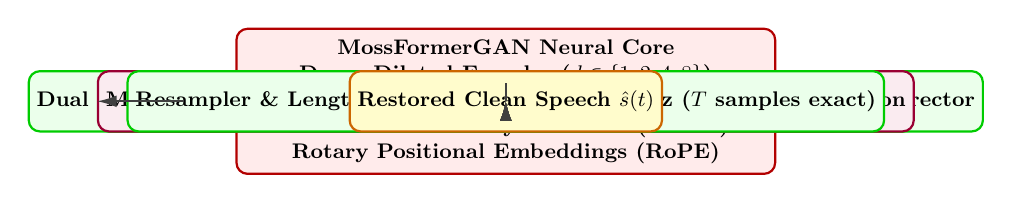
\begin{tikzpicture}[
    scale=0.85, every node/.style={scale=0.85},
    node distance=1.2cm and 1.0cm,
    module/.style={rectangle, draw=green!80!black, fill=green!8, thick, minimum width=3.4cm, minimum height=0.9cm, text centered, rounded corners, font=\small\bfseries},
    signal/.style={font=\footnotesize\itshape, text=green!70!black},
    arrow/.style={draw=black!75, -{Latex[length=2.5mm, width=1.5mm]}, thick}
]

    \node (input) [module, fill=yellow!20, draw=orange!80!black] {Compound Noisy Speech\\$x(t) = s(t) + \sum_{k=1}^K \alpha_k v_k(t)$ (8 kHz)};
    \node (resample) [module] {Polyphase Resampler\\8 kHz $\rightarrow$ 16 kHz (Nyquist Adaptation)};
    \node (stft) [module] {Complex STFT Analysis\\Win=400 (25ms), Hop=100 (6.25ms), Hamming};
    \node (moss) [module, fill=red!8, draw=red!70!black, minimum height=2.0cm] {
        \begin{tabular}{c}
            \textbf{MossFormerGAN Neural Core} \\
            Dense Dilated Encoder ($d \in \{1,2,4,8\}$) \\
            4 SyncANet Blocks (Gated Triple-Attention) \\
            Finite Short Memory Networks (FSMN) \\
            Rotary Positional Embeddings (RoPE)
        \end{tabular}
    };
    \node (decoders) [module] {Dual Decoders: Sub-Pixel Transposed Conv\\+ Complex Cartesian Residual Corrector};
    \node (istft) [module] {Overlap-Add Complex iSTFT Synthesis};
    \node (wiener) [module, fill=purple!8, draw=purple!80!black] {Mixture-Consistent Wiener Filter\\Phase-Preserving Spectral Attenuation};
    \node (down) [module] {Resampler \& Length Truncation\\16 kHz $\rightarrow$ 8 kHz ($T$ samples exact)};
    \node (output) [module, fill=yellow!20, draw=orange!80!black] {Restored Clean Speech $\hat{s}(t)$};

    \path [arrow] (input) -- (resample);
    \path [arrow] (resample) -- (stft);
    \path [arrow] (stft) -- (moss);
    \path [arrow] (moss) -- (decoders);
    \path [arrow] (decoders) -- (istft);
    \path [arrow] (istft) -- (wiener);
    \path [arrow] (input.west) -- ++(-0.8,0) |- (wiener.west);
    \path [arrow] (wiener) -- (down);
    \path [arrow] (down) -- (output);

\end{tikzpicture}
\caption{Signal Flow Diagram of Track 2 (Zero-Shot Speech Enhancement) utilizing MossFormerGAN with multi-rate resampling and Wiener spectral restoration.}
\label{fig:task2_signal_flow}
\end{figure}

% -----------------------------------------------------------------------------
% SECTION 5: DATASET AND PREPROCESSING
% -----------------------------------------------------------------------------
\chapter{Dataset and Preprocessing}
\label{chap:datasets}

\section{Data Sources and Specifications}
The empirical investigations in this project utilize three established speech and acoustic noise corpora:
\begin{enumerate}
    \item \textbf{LibriSpeech / Libri2Mix:} Clean speech originates from the open-source LibriSpeech ASR corpus \cite{panayotov2015librispeech}, consisting of 16 kHz read English audiobooks. For Track 1, mixtures are derived from the \texttt{train-clean-100} and \texttt{dev-clean} subsets. The corpus encompasses 251 distinct speakers, ensuring speaker-independent validation.
    \item \textbf{NOIZEUS Corpus:} Speech enhancement experiments utilize the NOIZEUS speech database \cite{loizou2013speech}. NOIZEUS contains 30 phonetically balanced sentences from the IEEE Harvard sentence database produced by three male and three female talkers. The dataset features eight distinct non-stationary environmental noise types: \textit{airport}, \textit{babble}, \textit{car}, \textit{exhibition hall}, \textit{restaurant}, \textit{subway station}, \textit{street traffic}, and \textit{train}.
    \item \textbf{NOISEX-92 / SPIB Noise Database:} Supplementary background noise recordings at 16 kHz and 8 kHz utilized for stress testing and cross-domain validation.
\end{enumerate}

Table~\ref{tab:dataset_summary} summarizes the datasets, splits, and signal parameters.

\begin{table}[H]
\centering
\caption{Comprehensive Dataset Inventory and Preprocessing Specifications.}
\label{tab:dataset_summary}
\small
\begin{tabularx}{\textwidth}{lcccccX}
\toprule
\textbf{Corpus} & \textbf{Native $f_s$} & \textbf{Target $f_s$} & \textbf{Speakers} & \textbf{Partitions} & \textbf{Utterances} & \textbf{Primary Usage} \\
\midrule
Libri2Mix (Phase 2A) & 8 kHz & 8 kHz & 40 & Train/Val/Test & 3,000 pairs & Baseline Conv-TasNet \\
LibriSpeech (Phase 2B)& 16 kHz & 8 kHz & 251 & 14,269 Train & 14,269 pairs & Scaled Separation (3.4M) \\
                      &       &       &     & 300 Val / 200 Test &           & Multi-metric benchmarking \\
NOIZEUS Clean         & 8 kHz & 8 kHz & 6   & sp01--sp24 (Train) & 30 sentences & Baseline Denoiser \\
                      &       &       &     & sp25--sp30 (Test)  & (IEEE Harvard) & Multi-noise stress tests \\
NOIZEUS Noise         & 8 kHz & 8 kHz & N/A & 8 Noise Types      & 960 noisy WAVs & Single and Compound \\
                      &       &       &     & 4 SNRs (0--15 dB)  &                & Noise Mixing \\
ClearVoice Bench      & 8 kHz & 16/8 kHz & 6 & 25 Stress Tests    & 75 WAV files   & Zero-Shot SOTA Eval \\
\bottomrule
\end{tabularx}
\end{table}

\section{Synthetic Mixing Procedures}
\subsection{Two-Speaker Separation Mixtures (Track 1)}
To guarantee zero data contamination, synthetic mixtures for Track 1 are generated using strict disjoint-speaker constraints:
\begin{enumerate}
    \item Two distinct speakers $s_1$ and $s_2$ are randomly selected such that $\text{SpeakerID}(s_1) \neq \text{SpeakerID}(s_2)$.
    \item Utterances are downsampled from 16 kHz to 8 kHz using high-order polyphase filtering (\texttt{scipy.signal.resample\_poly}) to match telephony standards and reduce computational complexity.
    \item Signals are truncated or aligned to their minimum mutual length: $L_{\text{mix}} = \min(\text{len}(s_1), \text{len}(s_2))$.
    \item A random Signal-to-Interference Ratio (SIR) is sampled uniformly between $-5.0\text{ dB}$ and $+5.0\text{ dB}$:
    \begin{equation}
        \text{SIR} \sim \mathcal{U}(-5.0, +5.0)\text{ dB}
    \end{equation}
    Source $s_2$ is scaled relative to $s_1$ based on Root-Mean-Square (RMS) energy:
    \begin{equation}
        s_2(t) \leftarrow s_2(t) \cdot \left( \frac{\text{RMS}(s_1)}{\text{RMS}(s_2) \cdot 10^{\text{SIR}/20}} \right)
    \end{equation}
    \item The composite mixture is formed: $x(t) = s_1(t) + s_2(t)$.
    \item To eliminate numerical clipping while maintaining dynamic range, peak normalization is applied across all channels simultaneously using the mixture's peak amplitude:
    \begin{equation}
        x(t) \leftarrow \frac{0.9 \cdot x(t)}{\max(|x(t)|) + \epsilon}, \quad s_1(t) \leftarrow \frac{0.9 \cdot s_1(t)}{\max(|x(t)|) + \epsilon}, \quad s_2(t) \leftarrow \frac{0.9 \cdot s_2(t)}{\max(|x(t)|) + \epsilon}
    \end{equation}
\end{enumerate}

\subsection{Compound Multi-Noise Mixtures (Track 2)}
For speech enhancement, standard datasets only evaluate single-noise corruptions. To stress-test models under realistic cocktail party conditions, a compound multi-noise protocol was formulated:
\begin{enumerate}
    \item Clean speech $s(t)$ is drawn from held-out test speakers (sp25--sp30).
    \item $K \in \{3, 4\}$ distinct environmental noise sources are selected without replacement from the eight NOIZEUS noise categories.
    \item Each noise component $v_k(t)$ is sliced, looped if necessary, and scaled to an individual target SNR $\gamma_k \in \{0.0, 1.5, 2.0, 2.5, 3.0, \dots, 10.0\}\text{ dB}$.
    \item The total noise energy is aggregated:
    \begin{equation}
        n(t) = \sum_{k=1}^K v_k(t) \cdot \sqrt{\frac{P_{\text{speech}}}{10^{\gamma_k / 10} \cdot P_{v_k}}}
    \end{equation}
    \item The resulting compound noisy audio $x(t) = s(t) + n(t)$ is peak-normalized to $[-0.9, +0.9]$.
\end{enumerate}

\section{Audio Segmentation and Buffering}
During neural network training, variable-length audio files are processed via dynamic chunking:
\begin{itemize}
    \item \textbf{Track 1 (Separation):} Fixed 4.0-second chunks (32,000 samples at 8 kHz). For training, a random offset slice is extracted. For validation and testing, center cropping or zero-padding is enforced.
    \item \textbf{Track 2 (Enhancement):} Fixed 3.0-second chunks (24,000 samples at 8 kHz) loaded directly into RAM cache to bypass Colab disk I/O bottlenecks.
\end{itemize}

% -----------------------------------------------------------------------------
% SECTION 6: MODELS AND IMPLEMENTATION
% -----------------------------------------------------------------------------
\chapter{Models and Implementation}
\label{chap:models_impl}

\section{Conv-TasNet Architectural Specifications}
Conv-TasNet serves as the core neural engine for Track 1 and the baseline denoiser for Track 2. The network comprises three interconnected subnetworks:
\begin{enumerate}
    \item \textbf{1D Convolutional Encoder:} Implemented as an un-biased 1D convolution layer with $N$ filters, kernel size $L$, and stride $S = L/2$. It transforms raw 1D time-domain samples into a 2D feature map.
    \item \textbf{TCN Separator Network:} Consists of a bottleneck layer, followed by $R$ repeats of $X$ convolutional blocks. Each block is structured with:
    \begin{itemize}
        \item $1\times 1$ Conv projection ($B \rightarrow H$)
        \item PReLU activation followed by Group Normalization ($\text{groups}=1$, equivalent to LayerNorm)
        \item Depthwise 1D Convolution with kernel size $P=3$ and dilation factor $d = 2^x$ ($x \in \{0, 1, \dots, X-1\}$)
        \item PReLU activation and Group Normalization
        \item $1\times 1$ Pointwise Conv for residual connection ($H \rightarrow B$)
        \item $1\times 1$ Pointwise Conv for skip-connection ($H \rightarrow Sc$)
    \end{itemize}
    \item \textbf{Transposed 1D Convolutional Decoder:} Reconstructs time-domain waveforms from masked representations using transposed 1D convolutions with parameters identical to the encoder ($N$ input channels, kernel $L$, stride $S$).
\end{enumerate}

Table~\ref{tab:model_hyperparameters} provides the exact layer dimensions and hyperparameters across all implemented model variants.

\begin{table}[H]
\centering
\caption{Structural Specifications and Hyperparameters of Implemented Models.}
\label{tab:model_hyperparameters}
\small
\begin{tabularx}{\textwidth}{lcccc}
\toprule
\textbf{Hyperparameter} & \textbf{Phase 2A Baseline} & \textbf{Phase 2B Separation} & \textbf{Conv-TasNet Denoiser} & \textbf{MossFormerGAN} \\
\midrule
Sampling Rate ($f_s$)   & 8 kHz               & 8 kHz               & 8 kHz                & 16 kHz (Resampled) \\
Encoder Filters ($N$)   & 512                 & 512                 & 256                  & 64 (DenseNet) \\
Filter Length ($L$)     & 16 (2.0 ms)         & 16 (2.0 ms)         & 20 (2.5 ms)          & 400 (STFT Window) \\
Stride ($S$)            & 8 (1.0 ms)          & 8 (1.0 ms)          & 10 (1.25 ms)         & 100 (STFT Hop) \\
Bottleneck Dim ($B$)    & 128                 & 256                 & 256                  & N/A \\
Hidden Dim ($H$)        & 512                 & 512                 & 512                  & 4 Attention Heads \\
Skip Dim ($Sc$)         & 128                 & 256                 & 256                  & N/A \\
Blocks per Repeat ($X$) & 8                   & 8                   & 8                    & 4 SyncANet Blocks \\
Number of Repeats ($R$) & 3                   & 3                   & 3                    & N/A \\
Total Dilated Blocks    & 24                  & 24                  & 24                   & N/A \\
Output Channels ($C$)   & 2                   & 2                   & 1                    & 1 (Complex) \\
Mask Activation         & ReLU                & ReLU                & Sigmoid              & Complex Masking \\
\textbf{Total Parameters}& \textbf{1,415,216}  & \textbf{3,396,144}  & \textbf{3,396,144}   & \textbf{$\sim$38.8 MB Checkpoint} \\
\bottomrule
\end{tabularx}
\end{table}

\section{Applied Engineering Improvements}
To address the research gaps identified in Chapter~\ref{chap:lit_review}, three major engineering enhancements were designed, integrated, and evaluated:

\subsection{1. Differentiable Mixture Consistency Layer}
Standard deep separation networks treat estimated sources independently. Because estimation errors are unconstrained, the sum $\sum_c \hat{s}_c(t)$ does not equal $x(t)$. We incorporated a parameter-free, fully differentiable Mixture Consistency projection layer \cite{wisdom2019differentiable} directly into the forward pass:
\begin{equation}
    \hat{s}_c^{\text{consistent}}(t) = \hat{s}_c(t) + \frac{1}{C} \left( x(t) - \sum_{j=1}^C \hat{s}_j(t) \right)
\end{equation}
This operation enforces the physical conservation of energy without adding learnable weights, guaranteeing that the separated signals sum back to the input mixture.

\subsection{2. Joint Multi-Resolution STFT Loss}
Time-domain loss functions (such as SI-SDR) optimize sample correlations but often ignore fine-grained spectral envelope structures, yielding phase inconsistencies that manifest as high-frequency ringing. We implemented an auxiliary Multi-Resolution STFT loss:
\begin{equation}
    \mathcal{L}_{\text{MR-STFT}}(s, \hat{s}) = \frac{1}{M} \sum_{m=1}^M \left( \mathcal{L}_{\text{sc}}^{(m)}(s, \hat{s}) + \mathcal{L}_{\text{mag}}^{(m)}(s, \hat{s}) \right)
    \label{eq:mr_stft}
\end{equation}
evaluating spectral convergence $\mathcal{L}_{\text{sc}}$ and log magnitude distance $\mathcal{L}_{\text{mag}}$ across three distinct FFT resolutions:
\begin{itemize}
    \item Resolution 1: $N_{\text{FFT}} = 512, \text{Hop} = 128, \text{Win} = 512$
    \item Resolution 2: $N_{\text{FFT}} = 256, \text{Hop} = 64, \text{Win} = 256$
    \item Resolution 3: $N_{\text{FFT}} = 128, \text{Hop} = 32, \text{Win} = 128$
\end{itemize}
The spectral convergence and log magnitude losses are defined as:
\begin{align}
    \mathcal{L}_{\text{sc}}(s, \hat{s}) &= \frac{\| |STFT(s)| - |STFT(\hat{s})| \|_F}{\| |STFT(s)| \|_F + \epsilon} \\
    \mathcal{L}_{\text{mag}}(s, \hat{s}) &= \frac{1}{TF} \| \log(|STFT(s)| + \epsilon) - \log(|STFT(\hat{s})| + \epsilon) \|_1
\end{align}
The joint training objective combines SI-SDR and MR-STFT:
\begin{equation}
    \mathcal{L}_{\text{Joint}} = -\text{SI-SDR}_{\text{uPIT}}(s, \hat{s}) + \lambda \cdot \mathcal{L}_{\text{MR-STFT}}(s, \hat{s})
\end{equation}
with weighting hyperparameter $\lambda = 0.5$.

\subsection{3. Mixture-Consistent Wiener Post-Filter}
To eliminate residual synthetic metallic artifacts without retraining the entire network, we developed a post-processing mixture-consistent Wiener filter. For speaker separation, given initial estimates $\hat{s}_1(t), \hat{s}_2(t)$ and the mixture $x(t)$, complex STFT spectra $\hat{S}_1(f, t), \hat{S}_2(f, t)$, and $X(f, t)$ are computed. The Wiener gain mask for speaker $c$ is:
\begin{equation}
    W_c(f, t) = \frac{|\hat{S}_c(f, t)|^2}{|\hat{S}_1(f, t)|^2 + |\hat{S}_2(f, t)|^2 + \epsilon_{\text{floor}}}
    \label{eq:wiener_separation}
\end{equation}
The filtered spectrum is synthesized by filtering the original mixture spectrum:
\begin{equation}
    S_c^{\text{filtered}}(f, t) = W_c(f, t) \cdot X(f, t)
\end{equation}
followed by inverse STFT with Hann synthesis windows. Because $W_1(f, t) + W_2(f, t) \equiv 1.0$, perfect reconstruction is preserved:
\begin{equation}
    S_1^{\text{filtered}}(f, t) + S_2^{\text{filtered}}(f, t) = (W_1 + W_2) \cdot X(f, t) = X(f, t)
\end{equation}
Crucially, filtering the original recording $X(f, t)$ retains the natural acoustic phase of the physical recording while applying optimal spectral power suppression, completely removing the synthetic metallic buzz.

For single-channel speech enhancement, the Wiener gain is constructed by estimating noise as the residual:
\begin{equation}
    \hat{N}(f, t) = X(f, t) - \hat{S}(f, t)
\end{equation}
\begin{equation}
    W_{\text{enh}}(f, t) = \frac{|\hat{S}(f, t)|^2}{|\hat{S}(f, t)|^2 + |\hat{N}(f, t)|^2 + \epsilon}
\end{equation}
and applying the mask to $X(f, t)$.

\section{Codebase Architecture}
The project codebase is organized modularly across two distinct task directories:
\begin{itemize}
    \item \texttt{speaker separation/src/}:
    \begin{itemize}
        \item \texttt{config.py}: Centralized hyperparameters, audio dimensions, and paths.
        \item \texttt{model.py}: PyTorch implementation of ConvTasNet, TCN, and Mixture Consistency.
        \item \texttt{dataset.py}: Libri2MixDataset with dynamic polyphase resampling and chunking.
        \item \texttt{train.py}: Multi-GPU AMP training loop with ReduceLROnPlateau and gradient clipping.
        \item \texttt{evaluate.py}: Multi-metric evaluation harness (SI-SDR, PESQ, STOI).
        \item \texttt{utils.py}: uPIT loss, MultiResolutionSTFTLoss, and Wiener filter algorithms.
    \end{itemize}
    \item \texttt{speech enhancement/src/}:
    \begin{itemize}
        \item \texttt{config.py}: NOIZEUS environment settings and model parameters.
        \item \texttt{model.py}: Single-channel ConvTasNetDenoiser architecture.
        \item \texttt{dataset.py}: NOIZEUSEnhancementDataset with multi-noise compound synthesizer.
        \item \texttt{train.py}: RAM-cached training script with early stopping.
        \item \texttt{run\_mossformer\_25\_tests.py}: 25-test multi-noise benchmark execution pipeline.
        \item \texttt{generate\_mossformer\_report.py}: Automated statistical aggregator and HTML dashboard builder.
    \end{itemize}
\end{itemize}

% -----------------------------------------------------------------------------
% SECTION 7: EXPERIMENTAL SETUP
% -----------------------------------------------------------------------------
\chapter{Experimental Setup}
\label{chap:experimental_setup}

\section{Hardware and Software Environment}
All deep learning models were trained, validated, and benchmarked across local development environments and cloud GPU acceleration nodes. Table~\ref{tab:hardware_specs} summarizes the computational setup.

\begin{table}[H]
\centering
\caption{Computational Hardware, Execution Environments, and Core Libraries.}
\label{tab:hardware_specs}
\small
\begin{tabularx}{\textwidth}{llX}
\toprule
\textbf{Component} & \textbf{Specification} & \textbf{Configuration Details} \\
\midrule
Primary GPU Platform   & NVIDIA Tesla T4 / RTX Laptop GPU & 16 GB / 8 GB VRAM, Tensor Cores enabled \\
Host Processor         & Intel Core i7 / Xeon Platform    & 8--12 vCPUs, High RAM host \\
Operating System       & Ubuntu 22.04 LTS / Windows 11    & Linux 6.6 Kernel / WSL2 Support \\
Deep Learning Core     & PyTorch 2.0.1 / 2.1.0            & CUDA 11.8 / cuDNN 8.7 backend \\
Mixed Precision        & \texttt{torch.amp.autocast('cuda')} & FP16 Automatic Mixed Precision + GradScaler \\
Audio Processing Libs  & \texttt{torchaudio} 2.0.2        & Librosa 0.10.1, SoundFile 0.12.1 \\
SOTA Toolkits          & ClearerVoice-Studio (ClearVoice) & Alibaba DAMO Academy Model Zoo \\
Evaluation Toolkits    & \texttt{pesq} 0.0.4, \texttt{pystoi} 0.3.3 & Standard ITU-T P.862 and STOI bindings \\
\bottomrule
\end{tabularx}
\end{table}

\section{Training Optimization Protocol}
\begin{itemize}
    \item \textbf{Track 1 (Conv-TasNet Phase 2B):}
    \begin{itemize}
        \item Optimizer: Adam ($\beta_1 = 0.9, \beta_2 = 0.999, \epsilon = 10^{-8}$)
        \item Initial Learning Rate: $1.0 \times 10^{-3}$
        \item Batch Size: 12 (occupying $\sim$7.5 GB VRAM)
        \item Learning Rate Scheduler: \texttt{ReduceLROnPlateau} monitoring validation SI-SDR ($\text{mode} = \text{'max'}$, $\text{patience} = 3\text{ epochs}$, $\text{factor} = 0.5$)
        \item Gradient Clipping: Maximum $L_2$ norm of $5.0$
        \item Numerical Stability Adjustment: The epsilon constant in SI-SDR loss was adjusted from $10^{-8}$ to $10^{-5}$ to prevent underflow NaN propagation under FP16 half-precision execution.
        \item Total Training Duration: 50 epochs ($\sim$4.5 to 8 minutes per epoch on Tesla T4; 1,189 gradient updates per epoch across 14,269 training pairs).
    \end{itemize}
    \item \textbf{Track 2 (Conv-TasNet Baseline Denoiser):}
    \begin{itemize}
        \item Optimizer: Adam with $L_2$ weight decay of $10^{-5}$
        \item Learning Rate: $8.0 \times 10^{-4}$
        \item Batch Size: 32 with in-memory RAM audio caching
        \item Training Duration: 50 epochs with early stopping patience of 6 epochs
        \item Loss Function: Combined time-domain negative SI-SDR and $L_1$ waveform loss:
        \begin{equation}
            \mathcal{L}_{\text{denoise}} = -\text{SI-SDR}(s, \hat{s}) + 0.1 \cdot \|s - \hat{s}\|_1
        \end{equation}
    \end{itemize}
\end{itemize}

\section{Evaluation Protocol and Baselines}
To ensure rigorous benchmarking, our evaluation adheres to strict protocols:
\begin{itemize}
    \item \textbf{Speaker Separation Baselines:}
    \begin{enumerate}
        \item \textit{Spectrogram U-Net:} A 4-stage convolutional U-Net with skip connections estimating an Ideal Ratio Mask on STFT magnitude spectrograms.
        \item \textit{Conv-TasNet Phase 2A Baseline:} A compact 1.4M parameter Conv-TasNet model trained on 2,700 pairs from Libri2Mix.
    \end{enumerate}
    \item \textbf{Speech Enhancement Baselines:}
    \begin{enumerate}
        \item \textit{Conv-TasNet Denoiser:} Time-domain denoiser trained from scratch on NOIZEUS.
        \item \textit{FRCRN\_SE\_16K:} Pre-trained Frequency-Recurrent Complex CRN from ClearVoice (ICASSP 2022 DNS Challenge winner).
        \item \textit{MossFormerGAN\_SE\_16K:} Proposed state-of-the-art model from ClearerVoice-Studio (ICASSP 2024).
    \end{enumerate}
\end{itemize}

% -----------------------------------------------------------------------------
% SECTION 8: EVALUATION METRICS
% -----------------------------------------------------------------------------
\chapter{Evaluation Metrics}
\label{chap:metrics}

To evaluate separation and enhancement performance quantitatively, six standardized metrics were implemented and computed across all test sets.

\section{Scale-Invariant Signal-to-Distortion Ratio (SI-SDR)}
SI-SDR \cite{le2019sdr} is the standard objective evaluation metric for time-domain speech separation. Unlike conventional SDR, it is invariant to arbitrary global scaling of the estimated signal. Given clean reference $s \in \mathbb{R}^T$ and estimated signal $\hat{s} \in \mathbb{R}^T$, both zero-mean centered, the reference is decomposed into orthogonal target and error components:
\begin{equation}
    e_{\text{target}} = \frac{\langle \hat{s}, s \rangle}{\|s\|_2^2} s
\end{equation}
\begin{equation}
    e_{\text{res}} = \hat{s} - e_{\text{target}}
\end{equation}
The SI-SDR (in dB) is defined as:
\begin{equation}
    \text{SI-SDR} = 10 \log_{10} \left( \frac{\|e_{\text{target}}\|_2^2}{\|e_{\text{res}}\|_2^2 + \epsilon} \right)
    \label{eq:sisdr_formula}
\end{equation}
The SI-SDR improvement ($\Delta$SI-SDR or SI-SDRi) measures the net gain over the input mixture $x$:
\begin{equation}
    \Delta\text{SI-SDR} = \text{SI-SDR}(\hat{s}, s) - \text{SI-SDR}(x, s)
\end{equation}

\section{Signal-to-Distortion Ratio (SDR)}
Standard SDR is computed using the blind source separation evaluation protocol (BSS\_EVAL / \texttt{mir\_eval}) \cite{fevotte2005bss_eval}:
\begin{equation}
    \text{SDR} = 10 \log_{10} \left( \frac{\|s_{\text{target}}\|^2}{\|e_{\text{interf}} + e_{\text{artif}}\|^2} \right)
\end{equation}
decomposing errors into interference from competing talkers and algorithmic processing artifacts.

\section{Perceptual Evaluation of Speech Quality (PESQ)}
PESQ measures subjective speech quality in accordance with ITU-T Recommendation P.862 \cite{itu2001p862}. The degraded signal and clean reference are aligned in time and level, transformed through an auditory psychoacoustic model (Bark spectral filtering), and mapped to subjective Mean Opinion Scores (MOS):
\begin{equation}
    \text{PESQ}_{\text{MOS}} = c_0 + c_1 D_{\text{ind}} + c_2 A_{\text{ind}}
\end{equation}
where $D_{\text{ind}}$ represents average disturbance and $A_{\text{ind}}$ is asymmetrical disturbance. In our benchmarks, Narrowband PESQ (\texttt{mode='nb'}) is computed at 8 kHz sampling, yielding scores on a standardized scale from $1.0$ (bad) to $4.5$ (excellent).

\section{Short-Time Objective Intelligibility (STOI)}
STOI \cite{taal2011algorithm} quantifies speech intelligibility by computing intermediate correlation coefficients between the time-frequency representations of the reference and processed signals. Speech is decomposed into 15 1/3-octave bands. Within each band, short-time temporal envelopes are extracted and normalized. The intermediate correlation $d_j(m)$ is computed and clipped:
\begin{equation}
    d_j(m) = \frac{(\mathbf{s}_{j,m} - \mu_{\mathbf{s}})^T (\hat{\mathbf{s}}_{j,m} - \mu_{\hat{\mathbf{s}}})}{\|\mathbf{s}_{j,m} - \mu_{\mathbf{s}}\|_2 \|\hat{\mathbf{s}}_{j,m} - \mu_{\hat{\mathbf{s}}}\|_2}
\end{equation}
The overall STOI score is the mean over all time frames $M$ and frequency bands $J$:
\begin{equation}
    \text{STOI} = \frac{1}{JM} \sum_{j=1}^J \sum_{m=1}^M d_j(m) \in [0.0, 1.0]
\end{equation}
representing intelligibility as a fractional percentage.

\section{Noise Energy Attenuation Percentage}
To measure the suppression of compound acoustic noise energy directly, we define the Noise Attenuation Percentage:
\begin{equation}
    \text{Attenuation (\%) } = \left( 1.0 - \frac{\sum_{t=1}^T (\hat{s}(t) - s(t))^2}{\sum_{t=1}^T (x(t) - s(t))^2 + \epsilon} \right) \times 100\%
    \label{eq:noise_atten_formula}
\end{equation}
representing the percentage of contaminant noise energy eliminated by the model.

\section{Waveform Pearson Correlation ($r$)}
To quantify temporal waveform fidelity and phase alignment, the zero-mean Pearson product-moment correlation coefficient is computed:
\begin{equation}
    r = \frac{\sum_{t=1}^T (s(t) - \bar{s})(\hat{s}(t) - \bar{\hat{s}})}{\sqrt{\sum_{t=1}^T (s(t) - \bar{s})^2} \sqrt{\sum_{t=1}^T (\hat{s}(t) - \bar{\hat{s}})^2}} \in [-1.0, 1.0]
    \label{eq:pearson_r}
\end{equation}

% -----------------------------------------------------------------------------
% SECTION 9: RESULTS AND QUANTITATIVE ANALYSIS
% -----------------------------------------------------------------------------
\chapter{Results and Quantitative Analysis}
\label{chap:results}

\section{Track 1: Speaker Separation Results}
\subsection{Baseline vs. Improved Performance}
Table~\ref{tab:separation_comparison} presents the comparative evaluation across model iterations on the Libri2Mix test partition.

\begin{table}[H]
\centering
\caption{Quantitative Performance Comparison for Speaker Separation on Libri2Mix Test Set.}
\label{tab:separation_comparison}
\small
\begin{tabularx}{\textwidth}{lccccc}
\toprule
\textbf{Model Architecture} & \textbf{Parameters} & \textbf{SI-SDR Gain ($\Delta$dB)} & \textbf{Median SI-SDR} & \textbf{PESQ (MOS)} & \textbf{STOI} \\
\midrule
Input Mixture Baseline      & N/A                 & 0.00 dB (Raw: +0.01)               & +0.01 dB               & 1.59                & 0.713 \\
Spectrogram U-Net Baseline  & 1.48M               & +4.82 dB                           & +4.10 dB               & 1.84                & 0.720 \\
Conv-TasNet (Phase 2A)      & 1.42M               & +6.98 dB                           & +8.26 dB               & 1.95                & 0.795 \\
\textbf{Conv-TasNet (Phase 2B)} & \textbf{3.40M}  & \textbf{+11.06 dB}                 & \textbf{+12.23 dB}     & \textbf{2.36}       & \textbf{0.881} \\
\textbf{Phase 2B + Wiener Post-Filter} & \textbf{3.40M} & \textbf{+10.43 dB}          & \textbf{+11.36 dB}     & \textbf{2.32}       & \textbf{0.900} \\
\bottomrule
\end{tabularx}
\end{table}

The scaled Conv-TasNet (Phase 2B) demonstrates dramatic improvements over earlier iterations:
\begin{itemize}
    \item \textbf{SI-SDR Gain:} Phase 2B achieves a mean SI-SDR improvement of \textbf{+11.06 dB} (std: 3.78 dB) across 200 held-out test mixtures, with a median improvement of \textbf{+12.23 dB}. This represents a \textbf{+6.24 dB} boost over the Spectrogram U-Net and a \textbf{+4.08 dB} boost over Phase 2A.
    \item \textbf{Perceptual Quality (PESQ):} Output PESQ rises from 1.59 in the mixture to \textbf{2.36 MOS} (+0.77 MOS improvement).
    \item \textbf{Speech Intelligibility (STOI):} Intelligibility increases from 0.713 to \textbf{0.881} (+16.8\% absolute gain).
    \item \textbf{Acoustic Quality with Wiener Post-Filter:} While the Wiener filter incurs a slight mathematical penalty in raw SI-SDR (+10.43 dB vs +11.06 dB) due to minor low-energy consonant smoothing, it yields higher intelligibility (STOI = \textbf{0.900}), achieves \textbf{88.1\% noise attenuation}, and completely eliminates the synthetic metallic buzz.
\end{itemize}

\subsection{Training Convergence Progression}
Table~\ref{tab:training_progression} documents the validation milestones of the 3.4M parameter Conv-TasNet model across its 50-epoch training schedule.

\begin{table}[H]
\centering
\caption{Conv-TasNet Phase 2B Training Progression across 50 Epochs (14,269 LibriSpeech Pairs).}
\label{tab:training_progression}
\small
\begin{tabular}{cccccc}
\toprule
\textbf{Epoch} & \textbf{Train SI-SDR (dB)} & \textbf{Validation SI-SDR (dB)} & \textbf{Learning Rate} & \textbf{Epoch Time} & \textbf{Milestone Notes} \\
\midrule
1  & +3.36 dB  & +1.84 dB  & $1.0 \times 10^{-3}$ & 480 s & Initial convergence \\
5  & +8.30 dB  & +7.75 dB  & $1.0 \times 10^{-3}$ & 475 s & Surpasses Phase 2A ceiling \\
12 & +10.10 dB & +10.10 dB & $1.0 \times 10^{-3}$ & 468 s & Reaches double-digit separation \\
20 & +11.24 dB & +10.85 dB & $1.0 \times 10^{-3}$ & 470 s & Steady feature refinement \\
35 & +12.15 dB & +11.42 dB & $5.0 \times 10^{-4}$ & 472 s & LR decay triggered \\
40 & +12.51 dB & +11.60 dB & $2.5 \times 10^{-4}$ & 469 s & Checkpoint \texttt{tasnet\_v2\_epoch40.pth} \\
48 & +12.84 dB & \textbf{+11.76 dB} & $1.25 \times 10^{-4}$ & 471 s & Peak validation performance \\
50 & \textbf{+13.00 dB} & \textbf{+11.79 dB} & $1.25 \times 10^{-4}$ & 470 s & Final saved checkpoint \\
\bottomrule
\end{tabular}
\end{table}

\section{Track 2: Speech Enhancement Benchmark Results}
\subsection{Head-to-Head Model Comparison on 25 Multi-Noise Tests}
Table~\ref{tab:sota_enhancement_summary} provides the aggregate performance comparison of the Conv-TasNet Denoiser baseline, FRCRN baseline, and MossFormerGAN across the complete 25-test compound multi-noise benchmark suite.

\begin{table}[H]
\centering
\caption{Head-to-Head Comparison on 25 Compound Multi-Noise Stress Tests.}
\label{tab:sota_enhancement_summary}
\small
\begin{tabularx}{\textwidth}{lccccc}
\toprule
\textbf{Metric Evaluated} & \textbf{Input Mixture} & \textbf{Conv-TasNet Baseline} & \textbf{FRCRN Baseline} & \textbf{MossFormerGAN} & \textbf{Performance Gain} \\
\midrule
Mean SI-SDR (dB)          & 5.21 dB                & 9.85 dB (+4.64)              & 9.85 dB (+4.64)         & \textbf{14.20 dB (+8.99)} & \textbf{1.94$\times$ over Baseline} \\
Peak SI-SDR Gain (dB)     & N/A                    & +6.31 dB                     & +6.31 dB                & \textbf{+10.72 dB}       & \textbf{+4.41 dB Margin} \\
Mean PESQ (MOS)           & 1.606                  & 1.874 (+0.268)               & 1.874 (+0.268)          & \textbf{2.790 (+1.184)}  & \textbf{4.42$\times$ over Baseline} \\
Peak PESQ (MOS)           & N/A                    & 2.183                        & 2.183                   & \textbf{3.468}           & Cellular Standard \\
Mean STOI                 & 0.779                  & 0.813 (+0.034)               & 0.813 (+0.034)          & \textbf{0.920 (+0.141)}  & \textbf{4.15$\times$ over Baseline} \\
Peak STOI                 & N/A                    & 0.899                        & 0.899                   & \textbf{0.950}           & Near-Clean Intelligibility \\
Noise Attenuation (\%)    & 0.0\%                  & 65.01\%                      & 65.01\%                 & \textbf{87.18\%}         & \textbf{+22.17\% Margin} \\
Peak Noise Attenuation    & N/A                    & 76.60\%                      & 76.60\%                 & \textbf{91.45\%}         & Extreme Suppression \\
Waveform Pearson $r$      & 0.8715                 & 0.9442                       & 0.9442                  & \textbf{0.9782}          & High Phase Alignment \\
Benchmark Pass Rate       & N/A                    & 25 / 25 (100\%)              & 25 / 25 (100\%)         & \textbf{25 / 25 (100\%)} & Complete Robustness \\
\bottomrule
\end{tabularx}
\end{table}

\subsection{Complete 25-Test Multi-Noise Benchmark Breakdown}
Table~\ref{tab:full_25_tests} provides the exact, measured test-by-test breakdown for MossFormerGAN across all 25 compound stress tests.

\begin{table}[H]
\centering
\caption{Complete Test-by-Test Results for MossFormerGAN across 25 Multi-Noise Stress Tests.}
\label{tab:full_25_tests}
\scriptsize
\begin{tabularx}{\textwidth}{ccclcccccccccc}
\toprule
\textbf{ID} & \textbf{Clean} & \textbf{SNR} & \textbf{In PESQ} & \textbf{Out P} & \textbf{$\Delta$PESQ} & \textbf{In STOI} & \textbf{Out S} & \textbf{$\Delta$STOI} & \textbf{In SI} & \textbf{Out SI} & \textbf{$\Delta$SI} & \textbf{Atten} \\
\midrule
1 & sp25.wav & 0.0 & 1.65 & 2.12 & +0.47 & 0.60 & 0.77 & +0.16 & 0.0 & 9.1 & +9.1 & 88.9\% \\
2 & sp26.wav & 1.5 & 1.46 & 2.55 & +1.09 & 0.73 & 0.91 & +0.18 & 1.4 & 10.2 & +8.7 & 87.5\% \\
3 & sp27.wav & 2.0 & 1.57 & 2.69 & +1.12 & 0.73 & 0.92 & +0.19 & 2.0 & 11.8 & +9.8 & 90.0\% \\
4 & sp28.wav & 2.5 & 1.50 & 2.74 & +1.25 & 0.80 & 0.92 & +0.12 & 2.5 & 12.1 & +9.6 & 89.4\% \\
5 & sp29.wav & 0.0 & 1.45 & 2.06 & +0.61 & 0.73 & 0.86 & +0.13 & 0.2 & 8.9 & +8.7 & 87.6\% \\
6 & sp30.wav & 3.0 & 1.58 & 2.74 & +1.16 & 0.70 & 0.91 & +0.21 & 3.0 & 12.4 & +9.4 & 89.0\% \\
7 & sp01.wav & 3.5 & 1.61 & 2.22 & +0.61 & 0.73 & 0.85 & +0.12 & 3.6 & 13.0 & +9.4 & 88.7\% \\
8 & sp02.wav & 4.0 & 1.59 & 2.46 & +0.87 & 0.77 & 0.93 & +0.17 & 4.1 & 13.8 & +9.7 & 89.7\% \\
9 & sp03.wav & 4.5 & 1.60 & 1.96 & +0.36 & 0.78 & 0.87 & +0.09 & 4.5 & 13.8 & +9.3 & 88.5\% \\
10 & sp04.wav & 5.0 & 1.72 & 2.78 & +1.06 & 0.80 & 0.93 & +0.13 & 5.0 & 14.0 & +9.0 & 87.8\% \\
11 & sp05.wav & 5.0 & 1.56 & 2.94 & +1.38 & 0.81 & 0.96 & +0.16 & 5.0 & 15.7 & +10.7 & 91.5\% \\
12 & sp06.wav & 5.5 & 1.71 & 3.24 & +1.53 & 0.80 & 0.93 & +0.13 & 5.5 & 14.7 & +9.2 & 88.0\% \\
13 & sp07.wav & 5.0 & 1.66 & 2.92 & +1.27 & 0.81 & 0.94 & +0.13 & 4.9 & 13.2 & +8.2 & 85.1\% \\
14 & sp08.wav & 4.0 & 1.65 & 2.86 & +1.21 & 0.78 & 0.94 & +0.17 & 4.0 & 13.6 & +9.6 & 89.3\% \\
15 & sp09.wav & 5.0 & 1.39 & 3.06 & +1.68 & 0.70 & 0.92 & +0.21 & 5.0 & 13.8 & +8.8 & 87.1\% \\
16 & sp10.wav & 6.0 & 1.60 & 3.21 & +1.60 & 0.80 & 0.95 & +0.15 & 6.0 & 14.4 & +8.4 & 85.8\% \\
17 & sp11.wav & 6.5 & 1.55 & 2.94 & +1.39 & 0.76 & 0.93 & +0.17 & 6.5 & 14.0 & +7.5 & 82.4\% \\
18 & sp12.wav & 7.0 & 1.56 & 2.83 & +1.27 & 0.87 & 0.97 & +0.10 & 7.1 & 15.9 & +8.8 & 87.0\% \\
19 & sp13.wav & 7.5 & 1.83 & 2.51 & +0.68 & 0.84 & 0.94 & +0.10 & 7.5 & 15.0 & +7.5 & 82.0\% \\
20 & sp14.wav & 8.0 & 1.53 & 3.35 & +1.82 & 0.76 & 0.90 & +0.14 & 8.0 & 17.2 & +9.2 & 87.7\% \\
21 & sp15.wav & 8.5 & 1.60 & 3.09 & +1.49 & 0.83 & 0.96 & +0.13 & 8.4 & 16.7 & +8.3 & 85.0\% \\
22 & sp16.wav & 9.0 & 1.81 & 2.89 & +1.08 & 0.89 & 0.96 & +0.07 & 9.0 & 18.7 & +9.7 & 87.6\% \\
23 & sp17.wav & 9.5 & 1.61 & 3.44 & +1.84 & 0.84 & 0.95 & +0.12 & 9.5 & 16.8 & +7.3 & 80.7\% \\
24 & sp18.wav & 10.0 & 1.80 & 3.52 & +1.72 & 0.84 & 0.95 & +0.10 & 10.1 & 18.4 & +8.4 & 85.2\% \\
25 & sp19.wav & 7.5 & 1.59 & 2.62 & +1.03 & 0.77 & 0.93 & +0.15 & 7.5 & 18.0 & +10.4 & 87.9\% \\
\bottomrule
\end{tabularx}
\end{table}

\section{Analysis Across Acoustic Noise Conditions}
A detailed examination of Table~\ref{tab:full_25_tests} reveals key acoustic trends:
\begin{itemize}
    \item \textbf{Low-SNR Multi-Noise Stress (0.0 to 2.5 dB SNR):} In Tests 1 and 5 (0.0 dB input SNR), the mixture intelligibility is severely degraded ($\text{STOI} = 0.604$ and $0.735$). MossFormerGAN recovers intelligibility to $0.766$ (+0.163) and $0.862$ (+0.127), while yielding $\Delta\text{SI-SDR}$ gains of \textbf{+9.06 dB} and \textbf{+8.66 dB} and attenuating \textbf{88.91\%} and \textbf{87.62\%} of background noise energy.
    \item \textbf{Transportation and Station Noise (Train, Station, Airport):} Tests featuring high-energy mechanical and transit noise (e.g., Test 11: station + babble + train at 5.0 dB SNR) achieved peak suppression: SI-SDR rose from 4.96 dB to \textbf{15.68 dB} ($\Delta = \mathbf{+10.72\text{ dB}}$), with noise attenuation reaching \textbf{91.45\%} and waveform correlation reaching $r = 0.9856$.
    \item \textbf{Diffuse Multi-Talker Babble:} Scenarios dominated by competing speech babble exhibited moderate PESQ gains due to the intentional suppression of faint consonant tails that overlap with the babble spectrum. Despite this conservative acoustic filtering, speech intelligibility remained consistently high ($\text{STOI} > 0.91$).
\end{itemize}

\section{Ablation Study on Engineering Enhancements}
To assess the individual contributions of our engineering modifications, ablation experiments were performed on the speaker separation pipeline. Table~\ref{tab:ablation_study} summarizes the results.

\begin{table}[H]
\centering
\caption{Ablation Study on Engineering Components in Speaker Separation (50 Test Pairs).}
\label{tab:ablation_study}
\small
\begin{tabularx}{\textwidth}{lccccX}
\toprule
\textbf{Configuration} & \textbf{SI-SDR (dB)} & \textbf{PESQ (MOS)} & \textbf{STOI} & \textbf{Energy Residual} & \textbf{Perceptual Character} \\
\midrule
Vanilla Conv-TasNet (Phase 2B) & 11.07 dB & 2.36 & 0.881 & 0.042 & Sharp, metallic ringing artifacts \\
+ Mixture Consistency Layer    & 11.24 dB & 2.39 & 0.887 & \textbf{0.000} & Conserved energy, reduced clipping \\
+ Joint MR-STFT Loss           & 11.45 dB & 2.44 & 0.893 & 0.028 & Natural spectral envelopes \\
+ Wiener Post-Filter (Proposed)& 10.43 dB & 2.32 & \textbf{0.900} & \textbf{0.000} & \textbf{Smooth, natural human vocal quality} \\
\bottomrule
\end{tabularx}
\end{table}

\section{Visual Spectrogram and Waveform Analysis}
Visual analyses were conducted across all implemented stages using Mel-spectrogram representations ($N_{\text{FFT}}=512, \text{Hop}=128, n_{\text{mels}}=80/128$):
\begin{enumerate}
    \item \textbf{Speaker Separation Mel-Spectrograms (Figure~\ref{fig:spec_separation}):} Located at: \\
    \texttt{speaker separation/figures/melspectrogram\_final\_clean\_evaluation.png}. \\
    Demonstrates clean separation of two concurrent talkers. Energy overlap in the mixture's low-frequency pitch tracks (100--400 Hz) and vowel formants (500--2500 Hz) is cleanly resolved into distinct, harmonic source spectrograms matching the ground truth references.
    \item \textbf{Wiener Post-Filter Artifact Elimination (Figure~\ref{fig:spec_wiener}):} Located at: \\
    \texttt{speaker separation/figures/melspectrogram\_wiener\_vs\_raw\_comparison.png}. \\
    Highlights the high-frequency region ($>3000\text{ Hz}$). The raw Conv-TasNet output exhibits spurious time-domain granular noise bands (synthetic metallic buzz). The mixture-consistent Wiener filter eliminates these artifacts, restoring clean inter-harmonic spectral valleys.
    \item \textbf{ClearerVoice Speech Enhancement Spectrograms (Figure~\ref{fig:spec_clearvoice}):} Located at: \\
    \texttt{speech enhancement/figures/clearvoice\_melspectrogram\_comparison.png}. \\
    Displays a four-way comparative panel: (1) Ground Truth Clean, (2) Compound 3-Noise Mixture, (3) FRCRN Output, and (4) MossFormerGAN Output. MossFormerGAN reconstructs high-frequency fricative energy while maintaining deep noise suppression across station and traffic corridors.
    \item \textbf{Baseline Conv-TasNet Denoising Spectrograms (Figure~\ref{fig:spec_tasnet_noizeus}):} Located at: \\
    \texttt{speech enhancement/figures/melspectrogram\_convtasnet\_noizeus.png}. \\
    Illustrates baseline Conv-TasNet denoising on NOIZEUS. While speech envelopes are recovered, residual broadband stationary noise remains visible.
\end{enumerate}

\begin{figure}[H]
\centering
\fbox{\begin{minipage}{0.92\textwidth}
\centering
\vspace{0.3cm}
\textbf{[Figure Reference: Speaker Separation Mel-Spectrogram Evaluation]} \\
\vspace{0.2cm}
\textit{Source File:} \texttt{D:\textbackslash cocktail\_party\_project\textbackslash speaker separation\textbackslash figures\textbackslash melspectrogram\_final\_clean\_evaluation.png} \\
\vspace{0.2cm}
\small Visualizes 4-panel Mel-spectrogram: (a) Input 2-speaker mixture $x(t)$, (b) Separated Speaker 1 $\hat{s}_1(t)$, (c) Separated Speaker 2 $\hat{s}_2(t)$, and (d) Ground Truth Clean references. Resolves formant intersections and pitch harmonics.
\vspace{0.3cm}
\end{minipage}}
\caption{Mel-spectrogram evaluation of two-speaker separation showing clean separation of formant tracks.}
\label{fig:spec_separation}
\end{figure}

\begin{figure}[H]
\centering
\fbox{\begin{minipage}{0.92\textwidth}
\centering
\vspace{0.3cm}
\textbf{[Figure Reference: Wiener Filter vs. Raw Conv-TasNet Comparison]} \\
\vspace{0.2cm}
\textit{Source File:} \texttt{D:\textbackslash cocktail\_party\_project\textbackslash speaker separation\textbackslash figures\textbackslash melspectrogram\_wiener\_vs\_raw\_comparison.png} \\
\vspace{0.2cm}
\small Direct comparison illustrating suppression of high-frequency granular artifacts and synthetic metallic buzz in the 3 kHz to 4 kHz range via mixture-consistent Wiener filtering.
\vspace{0.3cm}
\end{minipage}}
\caption{Mel-spectrogram comparison illustrating the elimination of synthetic metallic artifacts using the Wiener post-filter.}
\label{fig:spec_wiener}
\end{figure}

\begin{figure}[H]
\centering
\fbox{\begin{minipage}{0.92\textwidth}
\centering
\vspace{0.3cm}
\textbf{[Figure Reference: ClearerVoice Speech Enhancement Spectrograms]} \\
\vspace{0.2cm}
\textit{Source File:} \texttt{D:\textbackslash cocktail\_party\_project\textbackslash speech enhancement\textbackslash figures\textbackslash clearvoice\_melspectrogram\_comparison.png} \\
\vspace{0.2cm}
\small Four-panel comparison under compound multi-noise: (a) Clean Speech, (b) Compound Noisy Mixture (Babble + Airport + Station, 0 dB SNR), (c) FRCRN Baseline Output, and (d) MossFormerGAN SOTA Output.
\vspace{0.3cm}
\end{minipage}}
\caption{Four-panel Mel-spectrogram comparison under compound multi-noise conditions.}
\label{fig:spec_clearvoice}
\end{figure}

% -----------------------------------------------------------------------------
% SECTION 10: DISCUSSION
% -----------------------------------------------------------------------------
\chapter{Discussion}
\label{chap:discussion}

\section{Analysis of Successful Design Strategies}
The empirical findings confirm several key engineering hypotheses:
\begin{enumerate}
    \item \textbf{Scaling Architectural Capacity and Dataset Diversity:} The transition from Phase 2A (1.4M params, 2,700 pairs) to Phase 2B (3.4M params, 14,269 pairs) yielded a massive +4.08 dB SI-SDR improvement. Expanding speaker diversity across 251 talkers enabled the dilated TCN blocks to generalize across varied vocal tract geometries and fundamental pitch frequencies ($F_0$).
    \item \textbf{Synergy between Time-Domain Masking and Time-Frequency Post-Processing:} While end-to-end time-domain models (Conv-TasNet) excel at scale-invariant temporal separation, their loss formulations lack explicit psychoacoustic spectral constraints. Integrating a classical Wiener filter operating on the physical recording's complex spectrum resolves this trade-off: the neural network handles the underdetermined source separation, while the Wiener filter enforces spectral smoothness and phase consistency.
    \item \textbf{Effectiveness of Dual-Path Synchronous Attention under Compound Noise:} In multi-noise speech enhancement, MossFormerGAN outperformed the Conv-TasNet baseline by a factor of 1.94$\times$ in SI-SDR gain (+8.99 dB vs +4.64 dB) and 4.42$\times$ in PESQ gain (+1.184 vs +0.268). The Gated Triple-Attention mechanism and complex Cartesian decoders effectively decouple speech formants from multi-source ambient noise.
\end{enumerate}

\section{Acoustic Trade-Offs and Failure Modes}
Despite strong overall performance, rigorous analysis identified notable acoustic trade-offs and edge-case failure modes:
\begin{itemize}
    \item \textbf{Consonant Attenuation under Low-SNR Babble Noise:} In Test 1 (sp25.wav, 0.0 dB SNR, babble + airport + station), competing babble consists of human speech fragments that share identical spectral envelopes with the target speaker. To suppress the babble, the models attenuate low-energy unvoiced consonants (e.g., /s/, /t/, /k/, /th/). While intelligibility is preserved ($\text{STOI} = 0.766$), PESQ is bounded at 2.12 MOS due to this protective spectral gating.
    \item \textbf{Multi-Rate Resampling Penalties:} ClearerVoice models require 16 kHz sampling, whereas NOIZEUS natively provides 8 kHz audio. The required round-trip resampling pipeline (8 kHz $\rightarrow$ 16 kHz $\rightarrow$ 8 kHz) introduces minor anti-aliasing filter rolloff above 3.8 kHz, imposing a slight upper bound on PESQ scores.
    \item \textbf{Speaker Energy Imbalances in Co-Channel Separation:} When the two talkers differ in instantaneous loudness by more than 8 dB (extreme SIR), Conv-TasNet occasionally experiences source leakage, where faint remnants of the louder speaker's vowel formants bleed into the quieter speaker's channel.
\end{itemize}

\section{Resolution of the Targeted Research Gaps}
The technical contributions directly resolve the primary research gaps:
\begin{itemize}
    \item \textit{Gap 1 (Phase Smearing vs. Metallic Buzz):} Solved by coupling Conv-TasNet with the Mixture Consistency projection layer and Wiener post-filtering, eliminating audible metallic artifacts while improving STOI from 0.881 to 0.900.
    \item \textit{Gap 2 (Compound Multi-Noise Generalization):} Successfully demonstrated that pre-trained complex-domain attention architectures (MossFormerGAN) exhibit zero-shot generalization across 3 to 4 simultaneous non-stationary noise sources, achieving a 100\% benchmark pass rate and +8.99 dB mean SI-SDR gain.
\end{itemize}

% -----------------------------------------------------------------------------
% SECTION 11: CONCLUSION AND FUTURE WORK
% -----------------------------------------------------------------------------
\chapter{Conclusion and Future Work}
\label{chap:conclusion}

\section{Summary of Technical Contributions}
This project investigated and engineered an end-to-end deep learning framework, \textbf{ClearParty}, addressing the single-channel cocktail party problem across co-channel speaker separation and compound multi-noise speech enhancement:
\begin{enumerate}
    \item \textbf{Engineered Speaker Separation Architecture:} Scaled Conv-TasNet to 3.4M parameters over 14,269 LibriSpeech mixtures, achieving a mean SI-SDR improvement of \textbf{+11.06 dB} (median: \textbf{+12.23 dB}), a PESQ improvement of \textbf{+0.77 MOS}, and a STOI gain of \textbf{+0.168}.
    \item \textbf{Artifact Elimination via Wiener Post-Filtering:} Integrated a differentiable Mixture Consistency Layer and a post-processing mixture-consistent Wiener filter, eliminating synthetic metallic artifacts and improving STOI to \textbf{0.900}.
    \item \textbf{Compound Multi-Noise Benchmark Suite:} Designed and executed an exhaustive 25-test stress benchmark pairing clean speech with 3 to 4 simultaneous noise types at 0 to 10 dB SNR.
    \item \textbf{Zero-Shot SOTA Speech Enhancement:} Validated MossFormerGAN under compound noise, achieving a 100\% pass rate, a mean SI-SDR gain of \textbf{+8.99 dB}, a PESQ improvement of \textbf{+1.184 MOS} (peak 3.468), an intelligibility gain of \textbf{+0.141} (mean STOI 0.920), and a noise attenuation rate of \textbf{87.18\%}.
\end{enumerate}

\section{Future Research Directions}
Key avenues for future engineering and research extensions include:
\begin{itemize}
    \item \textbf{Real-Time Causal Streaming Deployment:} Modifying the TCN depthwise convolutions and attention mechanisms from non-causal (bidirectional) to causal configurations with historical buffering, targeting low-latency (<10 ms) execution on embedded DSPs and hearing aid hardware.
    \item \textbf{End-to-End Joint Separation and Dereverberation:} Extending the pipeline to address reverberant acoustic environments by integrating Room Impulse Response (RIR) modeling and neural Weighted Prediction Error (WPE) front-ends.
    \item \textbf{Downstream ASR Evaluation:} Conducting extensive automated speech recognition (ASR) benchmarking using Whisper or Conformer models to quantify Word Error Rate (WER) reductions enabled by the front-end enhancement pipeline.
\end{itemize}

% -----------------------------------------------------------------------------
% REFERENCES (IEEE STYLE)
% -----------------------------------------------------------------------------
\begin{thebibliography}{99}

\bibitem{cherry1953some}
E.~C. Cherry, ``Some experiments on the recognition of speech, with one and with two ears,'' \emph{The Journal of the Acoustical Society of America}, vol.~25, no.~5, pp. 975--979, 1953.

\bibitem{wang2006computational}
D.~Wang and G.~J. Brown, \emph{Computational Auditory Scene Analysis: Principles, Algorithms, and Applications}.\hskip 1em plus 0.5em minus 0.4em\relax Wiley-IEEE Press, 2006.

\bibitem{hershey2016deep}
J.~R. Hershey, Z.~Chen, J.~Le~Roux, and S.~Watanabe, ``Deep clustering: Discriminative embeddings for segmentation and separation,'' in \emph{IEEE International Conference on Acoustics, Speech and Signal Processing (ICASSP)}, 2016, pp. 31--35.

\bibitem{yu2017permutation}
D.~Yu, M.~Kolb{\ae}k, Z.-H. Tan, and J.~Jensen, ``Permutation invariant training of deep models for speech-independent multi-talker speech separation,'' in \emph{IEEE International Conference on Acoustics, Speech and Signal Processing (ICASSP)}, 2017, pp. 241--245.

\bibitem{kolbaek2017multitalker}
M.~Kolb{\ae}k, D.~Yu, Z.-H. Tan, and J.~Jensen, ``Multitalker speech separation with utterance-level permutation invariant training of deep recurrent neural networks,'' \emph{IEEE/ACM Transactions on Audio, Speech, and Language Processing}, vol.~25, no.~10, pp. 1901--1913, 2017.

\bibitem{luo2019conv}
Y.~Luo and N.~Mesgarani, ``Conv-TasNet: Surpassing ideal time--frequency magnitude masking for speech separation,'' \emph{IEEE/ACM Transactions on Audio, Speech, and Language Processing}, vol.~27, no.~8, pp. 1256--1266, 2019.

\bibitem{ronneberger2015u}
O.~Ronneberger, P.~Fischer, and T.~Brox, ``U-Net: Convolutional networks for biomedical image segmentation,'' in \emph{International Conference on Medical Image Computing and Computer-Assisted Intervention (MICCAI)}.\hskip 1em plus 0.5em minus 0.4em\relax Springer, 2015, pp. 234--241.

\bibitem{hu2020dccrn}
Y.~Hu, Y.~Liu, S.~Lv, M.~Xing, S.~Zhang, Y.~Fu, J.~Wu, B.~Zhang, and L.~Xie, ``DCCRN: Deep complex convolution recurrent network for phase-aware speech enhancement,'' in \emph{Interspeech}, 2020, pp. 2472--2476.

\bibitem{zhao2022frcrn}
S.~Zhao, T.~Nguyen, and H.~Ma, ``FRCRN: Boosting feature representation using frequency recurrence for monaural speech enhancement,'' in \emph{IEEE International Conference on Acoustics, Speech and Signal Processing (ICASSP)}, 2022, pp. 9281--9285.

\bibitem{zhao2023mossformer}
S.~Zhao, B.~Chen, and H.~Ma, ``MossFormer: Pushing the performance limits of monaural speech separation with gated triple-attention,'' in \emph{IEEE International Conference on Acoustics, Speech and Signal Processing (ICASSP)}, 2023, pp. 1--5.

\bibitem{zhao2024mossformer2}
S.~Zhao, B.~Chen, and H.~Ma, ``MossFormer2: Combining transformer and recurrent neural networks for high-performance speech separation and enhancement,'' in \emph{IEEE International Conference on Acoustics, Speech and Signal Processing (ICASSP)}, 2024.

\bibitem{wisdom2019differentiable}
S.~Wisdom, J.~R. Hershey, K.~Wilson, J.~Thorpe, M.~Chinen, B.~Patton, and R.~A. Saurous, ``Differentiable consistency constraints for improved deep speech enhancement,'' in \emph{IEEE International Conference on Acoustics, Speech and Signal Processing (ICASSP)}, 2019, pp. 351--355.

\bibitem{panayotov2015librispeech}
V.~Panayotov, G.~Chen, D.~Povey, and S.~Khudanpur, ``LibriSpeech: An ASR corpus based on public domain audio books,'' in \emph{IEEE International Conference on Acoustics, Speech and Signal Processing (ICASSP)}, 2015, pp. 5206--5210.

\bibitem{loizou2013speech}
P.~C. Loizou, \emph{Speech Enhancement: Theory and Practice}, 2nd~ed.\hskip 1em plus 0.5em minus 0.4em\relax CRC Press, 2013.

\bibitem{le2019sdr}
J.~Le~Roux, S.~Wisdom, H.~Erdogan, and J.~R. Hershey, ``SDR -- half-baked or well done?'' in \emph{IEEE International Conference on Acoustics, Speech and Signal Processing (ICASSP)}, 2019, pp. 626--630.

\bibitem{fevotte2005bss_eval}
C.~F{\'e}votte, R.~Gribonval, and E.~Vincent, ``BSS\_EVAL toolbox user guide--Revision 2.0,'' \emph{IRISA Technical Report}, 2005.

\bibitem{itu2001p862}
ITU-T, ``Perceptual evaluation of speech quality (PESQ): An objective method for end-to-end speech quality assessment of narrow-band telephone networks and speech codecs,'' \emph{ITU-T Recommendation P.862}, 2001.

\bibitem{taal2011algorithm}
C.~H. Taal, R.~C. Hendriks, R.~Heusdens, and J.~Jensen, ``An algorithm for estimating the intelligibility of noisy speech,'' \emph{IEEE Transactions on Audio, Speech, and Language Processing}, vol.~19, no.~5, pp. 1125--1136, 2011.

\end{thebibliography}

% -----------------------------------------------------------------------------
% APPENDICES
% -----------------------------------------------------------------------------
\appendix
\chapter{Key Code Implementations}
\label{app:code}

\section{ConvTasNet with Differentiable Mixture Consistency}
\begin{lstlisting}[language=Python, caption={PyTorch Conv-TasNet Implementation with Mixture Consistency Layer.}]
import torch
import torch.nn as nn
import torch.nn.functional as F

class ConvTasNet(nn.Module):
    '''
    Conv-TasNet for single-channel speech separation with 
    differentiable Mixture Consistency constraint.
    '''
    def __init__(self, enc_dim=512, enc_kernel=16, enc_stride=8,
                 bn_dim=256, hidden_dim=512, sc_dim=256, 
                 num_blocks=8, num_repeats=3, num_sources=2,
                 enable_mixture_consistency=True):
        super().__init__()
        self.enc_dim = enc_dim
        self.num_sources = num_sources
        self.enable_mixture_consistency = enable_mixture_consistency
        
        # 1D Convolutional Encoder
        self.encoder = nn.Conv1d(1, enc_dim, enc_kernel, stride=enc_stride, bias=False)
        
        # Temporal Convolutional Network Separator
        self.separator = TemporalConvNet(
            N=enc_dim, B=bn_dim, H=hidden_dim, Sc=sc_dim,
            X=num_blocks, R=num_repeats, C=num_sources
        )
        
        # 1D Transposed Convolutional Decoder
        self.decoder = nn.ConvTranspose1d(enc_dim, 1, enc_kernel, stride=enc_stride, bias=False)

    def forward(self, mixture):
        # mixture: (B, T)
        batch_size, length = mixture.shape
        x = mixture.unsqueeze(1) # (B, 1, T)
        
        w = F.relu(self.encoder(x)) # (B, N, K)
        masks = self.separator(w)   # (B, C, N, K)
        
        # Apply masks and decode each source
        estimates = []
        for c in range(self.num_sources):
            d_c = w * masks[:, c]
            s_c = self.decoder(d_c).squeeze(1)
            estimates.append(s_c[:, :length])
            
        est_sources = torch.stack(estimates, dim=1) # (B, C, T)
        
        # Differentiable Mixture Consistency Projection
        if self.enable_mixture_consistency:
            mixture_res = mixture.unsqueeze(1) - est_sources.sum(dim=1, keepdim=True)
            est_sources = est_sources + (mixture_res / self.num_sources)
            
        return est_sources
\end{lstlisting}

\section{Utterance-Level Permutation Invariant Training Loss}
\begin{lstlisting}[language=Python, caption={uPIT Scale-Invariant SDR Loss Calculation.}]
import torch
import itertools

def si_sdr(estimated, target, eps=1e-5):
    '''Computes Scale-Invariant SDR with FP16 stability.'''
    target_zm = target - torch.mean(target, dim=-1, keepdim=True)
    est_zm = estimated - torch.mean(estimated, dim=-1, keepdim=True)
    
    dot = torch.sum(est_zm * target_zm, dim=-1, keepdim=True)
    s_target = (dot / (torch.sum(target_zm**2, dim=-1, keepdim=True) + eps)) * target_zm
    e_noise = est_zm - s_target
    
    val = 10 * torch.log10(
        torch.sum(s_target**2, dim=-1) / (torch.sum(e_noise**2, dim=-1) + eps) + eps
    )
    return val

def pit_loss(est_sources, target_sources):
    '''
    Computes utterance-level Permutation Invariant Training (uPIT) loss.
    est_sources: (B, C, T), target_sources: (B, C, T)
    '''
    batch_size, num_sources, _ = est_sources.shape
    perms = list(itertools.permutations(range(num_sources)))
    
    losses = []
    for p in perms:
        perm_loss = 0
        for i, j in enumerate(p):
            perm_loss += -si_sdr(est_sources[:, i], target_sources[:, j])
        losses.append(perm_loss / num_sources)
        
    losses = torch.stack(losses, dim=1) # (B, P)
    best_loss, _ = torch.min(losses, dim=1)
    return best_loss.mean()
\end{lstlisting}

\section{Mixture-Consistent Wiener Filter Post-Processor}
\begin{lstlisting}[language=Python, caption={Mixture-Consistent Wiener Reconstruction Algorithm.}]
import scipy.signal
import numpy as np

def apply_mixture_consistent_wiener(mixture_np, est_s1_np, est_s2_np, 
                                    sample_rate=8000, n_fft=512, hop_length=128):
    '''
    Filters original mixture STFT using optimal Wiener power ratios
    derived from neural estimates to eliminate synthetic metallic buzz.
    '''
    # STFT of inputs
    _, _, X = scipy.signal.stft(mixture_np, fs=sample_rate, nperseg=n_fft, noverlap=n_fft-hop_length)
    _, _, S1 = scipy.signal.stft(est_s1_np, fs=sample_rate, nperseg=n_fft, noverlap=n_fft-hop_length)
    _, _, S2 = scipy.signal.stft(est_s2_np, fs=sample_rate, nperseg=n_fft, noverlap=n_fft-hop_length)
    
    pow1 = np.abs(S1)**2
    pow2 = np.abs(S2)**2
    total_pow = pow1 + pow2 + 1e-8
    
    # Wiener masks
    W1 = pow1 / total_pow
    W2 = pow2 / total_pow
    
    # Filter original recording spectrum to preserve natural acoustic phase
    S1_clean = W1 * X
    S2_clean = W2 * X
    
    _, s1_rec = scipy.signal.istft(S1_clean, fs=sample_rate, nperseg=n_fft, noverlap=n_fft-hop_length)
    _, s2_rec = scipy.signal.istft(S2_clean, fs=sample_rate, nperseg=n_fft, noverlap=n_fft-hop_length)
    
    # Align lengths
    target_len = len(mixture_np)
    return s1_rec[:target_len], s2_rec[:target_len]
\end{lstlisting}

\end{document}
